\subsection{The homomorphism F and the shift V}

Let A be a ring. In the rest of this paragraph, we denote respectively by + and × the addition and multiplication laws in W(A). We shall also write 0 for 0 \(_{A}\) and 1 for \(1_{A}\) . We define two maps \(^{1}\) \(F_{A}\) and \(V_{A}\) (also denoted simply by F and V) from W(A) into itself by the formulas

\begin{enumerate}
\def\labelenumi{(\arabic{enumi})}
\setcounter{enumi}{22}
\tightlist
\item
\end{enumerate}

\[
\mathrm{F} _ {\mathbf {A}} (\boldsymbol {a}) = \big (\mathrm{F} _ {n} (a _ {0},..., a _ {n + 1}) \big) _ {n \in \mathbb {N}},\tag{24}
\]

\[
\mathrm{V} _ {\mathrm{A}} (\boldsymbol {a}) = (0, a _ {0}, a _ {1}, \dots)
\]

\((\text{for } \boldsymbol{a} = (a_n)_{n \in \mathbb{N}} \text{ in } \mathrm{W(A)})\) . The map \(V_A\) is called the shift. The formula

\[
\Phi_ {n} \left(\mathrm{F} _ {0} (\boldsymbol {a}), \dots , \mathrm{F} _ {n} (\boldsymbol {a})\right) = \Phi_ {n + 1} \left(a _ {0}, \dots , a _ {n + 1}\right) \quad (n \in \mathbf {N})\tag{25}
\]

follows immediately from (15). It can also be written in the form

\[
\Phi_ {\mathrm{A}} \circ \mathrm{F} _ {\mathrm{A}} = f _ {\mathrm{A}} \circ \Phi_ {\mathrm{A}}.\tag{26}
\]

The formula

\[
\Phi_ {\mathrm{A}} \circ \mathrm{V} _ {\mathrm{A}} = v _ {\mathrm{A}} \circ \Phi_ {\mathrm{A}}\tag{27}
\]

follows from relation (3).

Let \(\rho : \mathbf{B} \to \mathbf{A}\) be a ring homomorphism. The relations

\begin{enumerate}
\def\labelenumi{(\arabic{enumi})}
\setcounter{enumi}{27}
\tightlist
\item
\end{enumerate}

\[
\mathbf {W} (\rho) \circ \mathrm{F} _ {\mathbf {B}} = \mathrm{F} _ {\mathbf {A}} \circ \mathbf {W} (\rho)\tag{29}
\]

\[
\mathrm{W} (\rho) \circ \mathrm{V} _ {\mathrm{B}} = \mathrm{V} _ {\mathrm{A}} \circ \mathrm{W} (\rho)
\]

follow immediately from the definitions.

PROPOSITION 3. — Let A be a ring.

\begin{enumerate}
\def\labelenumi{\alph{enumi})}
\item
  The map \(F_{A}\) is an endomorphism of the ring W(A).
\item
  The map \(V_{A}\) is an endomorphism of the additive group underlying the ring \(\mathbf{W}(\mathbf{A})\) .
\item
  For every a in W(A), one has \(F_{A}(V_{A}(a)) = p.a\) (sum in W(A) of p terms equal to a).
\item
  For all \(a\) and \(b\) in W(A), one has
\end{enumerate}

\begin{enumerate}
\def\labelenumi{(\arabic{enumi})}
\setcounter{enumi}{29}
\tightlist
\item
\end{enumerate}

\[
\mathrm{V} _ {\mathrm{A}} (a \times \mathrm{F} _ {\mathrm{A}} (b)) = \mathrm{V} _ {\mathrm{A}} (a) \times b\tag{31}
\]

\[
\mathrm{V} _ {\mathrm{A}} (a) \times \mathrm{V} _ {\mathrm{A}} (b) = p. \mathrm{V} _ {\mathrm{A}} (a \times b)
\]

(sum in W(A) of p terms equal to \(V_A(a \times b)\)).

\begin{enumerate}
\def\labelenumi{\alph{enumi})}
\setcounter{enumi}{4}
\tightlist
\item
  Set \(\mu = V_{A}(1) = (0, 1, 0, \ldots)\) . For every \(b\) in W(A), one has
\end{enumerate}

\[
\mathrm{V} _ {\mathrm{A}} \left(\mathrm{F} _ {\mathrm{A}} (\boldsymbol {b})\right) = \mu \times \boldsymbol {b}.\tag{32}
\]

\begin{enumerate}
\def\labelenumi{\alph{enumi})}
\setcounter{enumi}{5}
\tightlist
\item
  For every element \(\mathbf{a}\) of W(A), denote by \(\mathbf{a}^{*p}\) the product in W(A) of p elements equal to a. Then one has
\end{enumerate}

\[
\mathrm{F} _ {\mathbf {A}} (\boldsymbol {a}) \equiv \boldsymbol {a} ^ {* p} \bmod p. \mathrm{W} (\mathbf {A}) \quad (\text { ideal of } \mathrm{W} (\mathbf {A}) \text { generated by } p. \mathbf {1}).\tag{33}
\]

Let \(\rho: \mathbf{B} \to \mathbf{A}\) be a ring homomorphism satisfying the conditions of lemma 3 of no. 4. Then \(\mathbf{W}(\rho): \mathbf{W}(\mathbf{B}) \to \mathbf{W}(\mathbf{A})\) is a surjective ring homomorphism, and \(\Phi_{\mathbf{B}}: \mathbf{W}(\mathbf{B}) \to \mathbf{B}^{\mathbf{N}}\) is an injective ring homomorphism. Moreover, \(f_{\mathbf{B}}: \mathbf{B}^{\mathbf{N}} \to \mathbf{B}^{\mathbf{N}}\) is a ring homomorphism. By formulas (26) and (28), one has

\[
\Phi_ {\mathrm{B}} \circ \mathrm{F} _ {\mathrm{B}} = f _ {\mathrm{B}} \circ \Phi_ {\mathrm{B}}, \quad \mathrm{W} (\rho) \circ \mathrm{F} _ {\mathrm{B}} = \mathrm{F} _ {\mathrm{A}} \circ \mathrm{W} (\rho),
\]

whence assertion a) follows immediately. Assertion b) follows analogously from formulas (27) and (29) and from the fact that \(v_{B}\) is an endomorphism of the additive group underlying \(B^{N}\) .

Let \(\pmb{a}\) be an element of W(A), and choose an element \(\pmb{x}\) of W(B) whose image under W(ρ) is \(\pmb{a}\) . Put \(\xi = \Phi_{\mathrm{B}}(\pmb{x})\) . It follows immediately from the definitions of \(f_{\mathrm{B}}\) and \(v_{\mathrm{B}}\) that one has \(f_{\mathrm{B}}(v_{\mathrm{B}}(\xi)) = p.\xi\) (sum in B \(^{\mathbf{N}}\) of \(p\) terms equal to \(\xi\) ). By formulas (26) and (27) (where A is replaced by B), the elements F \(_{\mathrm{B}}\) (V \(_{\mathrm{B}}\) ( \(\pmb{x}\) )) and \(p.\pmb{x}\) of W(B) therefore have the same image \(p.\xi\) under the injective map \(\Phi_{\mathrm{B}}\) , and thus are equal. The formula F \(_{\mathrm{A}}\) (V \(_{\mathrm{A}}\) ( \(\pmb{a}\) )) = \(p.\pmb{a}\) then follows from relations (28) and (29). This proves \(c\) .

Reasoning analogously, one reduces the proof of formula (30) to that of the relation

\[
v _ {\mathrm{B}} (\xi f _ {\mathrm{B}} (\eta)) = v _ {\mathrm{B}} (\xi) \eta
\]

for \(\xi\) , \(\eta\) in B \(^{N}\) . Now this follows from the equalities

\[
\begin{array}{l} \xi f _ {\mathrm{B}} (\eta) = (\xi_ {0} \eta_ {1}, \xi_ {1} \eta_ {2}, \dots) \\ v _ {\mathrm{B}} (\xi) \eta = (0, p \xi_ {0} \eta_ {1}, p \xi_ {1} \eta_ {2}, \dots). \end{array}
\]

Taking (b) and (c) into account, formula (31) follows from formula (30), where \(\boldsymbol{b}\) is replaced by \(\mathrm{V}_{\mathbf{A}}(\boldsymbol{b})\) . Formula (32) is the particular case \(\boldsymbol{a} = \boldsymbol{1}\) of formula (30).

Similarly, one reduces the proof of formula (33) to that of the relation

\[
f _ {\mathrm{B}} (\xi) \equiv \xi^ {p} \bmod p. \Phi_ {\mathrm{B}} (\mathrm{B} ^ {\mathbf {N}}),
\]

where \(\xi^{p}\) denotes the product in \(\mathbf{B}^{\mathbf{N}}\) of \(p\) elements equal to \(\xi\) . By prop. 2, c) of no. 2, this is equivalent to the fact that for every \(n \geqslant 0\) , one has

\[
\sigma \left(\xi_ {n + 1} - \xi_ {n} ^ {p}\right) \equiv \xi_ {n + 2} - \xi_ {n + 1} ^ {p} \bmod p ^ {n + 2} \mathbf {B}.
\]

Now, for every \(n \geqslant 0\) , one has, by loc. cit.,

\[
\sigma (\xi_ {n}) \equiv \xi_ {n + 1} \bmod p ^ {n + 1} \mathbf {B}
\]

since \(\xi = \Phi_{\mathbf{B}}(\boldsymbol{x})\) ; from this one deduces, by means of lemma 1 of no. 1,

\[
\sigma (\xi_ {n}) ^ {p} \equiv \xi_ {n + 1} ^ {p} \bmod p ^ {n + 2} \mathbf {B}.
\]

This proves the desired relation.

Remark. --- For the definition of maps analogous to the maps F and V, in the case of the universal Witt ring, see exercises 36, 37 and 38, p. 52 and following.

\subsection{Filtration and topology of the ring W(A)}

Lemma 4. --- Let A be a ring and let \(m \geqslant 1\) be an integer. One has

\[
\boldsymbol {a} = \left(a _ {0}, \dots , a _ {m - 1}, 0, \dots\right) + \underbrace {\left(0 , \dots , 0 , \right.} _ {m \text { terms }}, a _ {m}, a _ {m + 1}, \dots)\tag{34}
\]

for all a in W(A).

Let \(\rho: B \to A\) be a ring homomorphism satisfying the conditions of lemma 3 of no. 4. Then \(W(\rho): W(B) \to W(A)\) is a surjective ring homomorphism, and \(\Phi_B: W(B) \to B^N\) is an injective homomorphism. It therefore suffices to prove that one has

\[
\Phi_ {n} (\boldsymbol {b}) = \Phi_ {n} (b _ {0},..., b _ {m - 1}, 0,...) + \Phi_ {n} (0,..., 0, b _ {m}, b _ {m + 1},...) \tag{35}
\]

for all b in W(B) and all integers \(m \geqslant 1, n \geqslant 0\) . Now one has

\[
\begin{array}{r l} \Phi_ {n} (b _ {0},..., b _ {m - 1},... \dots) & = \Phi_ {n} (b _ {0},..., b _ {n}) \quad \text { if } \quad 0 \leqslant n <   m \\ & = \sum_ {i = 0} ^ {m - 1} p ^ {i}. b _ {i} ^ {p ^ {n - i}} \quad \text { if } \quad m \leqslant n \end{array}
\]

\[
\begin{array}{r l} \Phi_ {n} (0, \dots , 0, b _ {m}, b _ {m + 1}, \dots) & = 0 \\ & = \sum_ {i = m} ^ {n} p ^ {i}. b _ {i} ^ {p ^ {n - i}} \end{array} \quad \text { if } \quad 0 \leqslant n <   m \quad \text { if } \quad m \leqslant n,
\]

whence formula (35).

Let A be a ring. For every integer \(m \geqslant 0\) , denote by \(\mathbf{V}_{m}(\mathbf{A})\) the set of Witt vectors \(\boldsymbol{a} = (a_{n})_{n \in \mathbb{N}}\) such that \(a_{n} = 0\) for \(0 \leqslant n < m\) . It is the image of the \(m\)-th power \(\mathbf{V}^{m}\) of the map \(\mathbf{V}_{\mathrm{A}}\) . The formulas

\begin{enumerate}
\def\labelenumi{(\arabic{enumi})}
\setcounter{enumi}{35}
\tightlist
\item
\end{enumerate}

\[
\mathrm{V} ^ {m} (\boldsymbol {a} + \boldsymbol {b}) = \mathrm{V} ^ {m} (\boldsymbol {a}) + \mathrm{V} ^ {m} (\boldsymbol {b})\tag{37}
\]

\[
\mathrm{V} ^ {m} (a) \times b = \mathrm{V} ^ {m} (a \times \mathrm{F} ^ {m} (b))
\]

result from prop. 3 of no. 5 by induction on m. They imply that V \(_{m}\) (A) is an ideal of W(A).

\pandocbounded{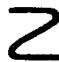
\includegraphics[keepaspectratio]{images/part001_18cee607.jpg}}

One sets \(\mathrm{V}_{m}(\mathrm{A}) = \mathrm{W}(\mathrm{A})\) if \(m < 0\) . The sequence \((\mathrm{V}_{m}(\mathrm{A}))_{m \in \mathbf{Z}}\) is a decreasing filtration on the additive group of the ring \(\mathrm{W}(\mathrm{A})\) . It is compatible with the ring structure of \(\mathrm{W}(\mathrm{A})\) (III, § 2, no. 1, def. 2) if and only if A is a ring of characteristic \(p\) (cf. no. 3, example 2 and infra, no. 8, corollary of prop. 5).

In what follows, one endows W(A) with the topology \(\mathcal{G}\) associated with the filtration \((\mathrm{V}_m(\mathrm{A}))_{m\in \mathbf{Z}}\) . Since \(\mathrm{V}_m(\mathrm{A})\) is an ideal of W(A) for all \(m\in \mathbf{Z}\) , the topology \(\mathcal{G}\) is compatible with the ring structure of W(A) (TG, III, p. 49, example 3). Let \(a\in \mathrm{W(A)}\) ; the sets \(a + \mathrm{V}_m(\mathrm{A})\) , where \(m\) runs through N, form a fundamental system of neighborhoods of \(a\) for \(\mathcal{G}\) . Now, it follows from lemma 4 that \(a + \mathrm{V}_m(\mathrm{A})\) consists of the Witt vectors \(b\) such that \(a_i = b_i\) for \(0\leqslant i < m\) . Consequently, \(\mathcal{G}\) is none other than the product topology on \(\mathbf{A}^{\mathbf{N}}\) of the discrete topology on each of the factors, and W(A) is therefore a separated and complete topological ring (TG, II, p. 17, prop. 10 and TG, III, p. 22, prop. 4).

Denote by \(\tau_{\mathbf{A}}\) (or simply \(\tau\) ) the map from A to W(A) which associates \((a, 0, 0, \ldots)\) with each element \(a\) of A. We have \(\Phi_n(\tau(a)) = a^{p^n}\) for every \(n \in \mathbb{N}\) . For every ring homomorphism \(\rho: \mathbf{B} \to \mathbf{A}\) , one has W( \(\rho\) ) \(\circ\) \(\tau_{\mathbf{B}} = \tau_{\mathbf{A}} \circ \rho\) .

PROPOSITION 4. --- Let \(a\) and \(b\) be in \(\mathbf{A}\) and let \(\boldsymbol{x} = (x_n)_{n \in \mathbb{N}}\) be an element of \(\mathbf{W}(\mathbf{A})\) .

\begin{enumerate}
\def\labelenumi{\alph{enumi})}
\tightlist
\item
  One has the formulas
\end{enumerate}

\begin{enumerate}
\def\labelenumi{(\arabic{enumi})}
\setcounter{enumi}{37}
\tightlist
\item
\end{enumerate}

\[
\tau (a b) = \tau (a) \times \tau (b)\tag{39}
\]

\[
\tau (a) \times x = (a ^ {p ^ {n}} x _ {n}) _ {n \in \mathbf {N}}.
\]

\begin{enumerate}
\def\labelenumi{\alph{enumi})}
\setcounter{enumi}{1}
\tightlist
\item
  The series with general term \(\mathbf{V}^{n}(\tau(x_{n}))\) is convergent in \(\mathbf{W}(\mathbf{A})\) , with sum \(x\) .
\end{enumerate}

Let \(n\) be a positive integer. The polynomial \(\mathbf{P}_{n}(\mathbf{X}_{0},\ldots,\mathbf{X}_{n};\mathbf{Y}_{0},\ldots,\mathbf{Y}_{n})\) introduced in no. 3 is isobaric of weight \(p^{n}\) in the family \((\mathbf{X}_{0},\ldots,\mathbf{X}_{n})\) when one assigns \(\mathbf{X}_{i}\) a weight \(p^{i}\) . One therefore has

\[
\mathrm{P} _ {n} \left(\mathrm{X} _ {0}, 0, \dots , 0; \mathrm{Y} _ {0}, \dots , \mathrm{Y} _ {n}\right) = \mathrm{X} _ {0} ^ {p ^ {n}} \mathrm{P} _ {n} (1, 0, \dots , 0; \mathrm{Y} _ {0}, \dots , \mathrm{Y} _ {n}).\tag{40}
\]

Since 1 = (1, 0, 0, \ldots) is the identity element of the ring of Witt vectors with coefficients in \(\mathbf{Z}[(X_n)_{n\in\mathbb{N}}, (Y_n)_{n\in\mathbb{N}}]\) , one has

\[
\mathrm{P} _ {n} (1, 0,..., 0; \mathrm{Y} _ {0},..., \mathrm{Y} _ {n}) = \mathrm{Y} _ {n}.\tag{41}
\]

By substituting \(a\) for \(\mathbf{X}_{0}\) and \(x_{i}\) for \(\mathbf{Y}_{i}\), we deduce from (40) and (41) the relation:

\[
\mathrm{P} _ {n} (a, 0, \dots , 0; x _ {0}, \dots , x _ {n}) = a ^ {p ^ {n}} x _ {n}.
\]

By the definition of multiplication in W(A), we have proved (39); formula (38) is a particular case of (39).

We prove \(b\) ). By definition, \(\mathbf{V}^{n}(\tau(x_{n}))\) is the sequence all of whose components are zero, except the one with index \(n\) which is equal to \(x_{n}\). It follows from Lemma 4, by induction on \(m\) that we have

\[
\sum_ {n = 0} ^ {m} \mathrm{V} ^ {n} (\tau (x _ {n})) = (x _ {0},..., x _ {m}, 0, 0,...)
\]

for every integer \(m \geqslant 0\) ; we deduce \(b\) ) by passing to the limit since the topology \(\mathcal{C}\) on W(A) is the product of the discrete topologies of the factors A.

\subsection{\texorpdfstring{The rings \(W_{n}(A)\) of Witt vectors of finite length}{The rings W\_\{n\}(A) of Witt vectors of finite length}}

DEFINITION 2.--- Let A be a ring and \(n \geqslant 1\) an integer. We denote by \(\mathbf{W}_{n}(\mathbf{A})\) the quotient ring \(\mathbf{W}(\mathbf{A}) / \mathbf{V}_{n}(\mathbf{A})\) .

Given elements \(a_0, \ldots, a_{n-1}\) of A, we denote \([a_0, \ldots, a_{n-1}]\) or \([a_i]_{0 \leq i < n}\) the class modulo \(\mathrm{V}_n(\mathrm{A})\) of the element \((a_0, \ldots, a_{n-1}, 0, 0, \ldots)\) of \(\mathrm{W}(\mathrm{A})\). By Lemma 4 of no. 6, the map \((a_0, \ldots, a_{n-1}) \mapsto [a_0, \ldots, a_{n-1}]\) from \(\mathrm{A}^n\) to \(\mathrm{W}_n(\mathrm{A})\) is a bijection. For this reason, one says that the elements of \(\mathrm{W}_n(\mathrm{A})\) are the Witt vectors of length \(n\) ; by analogy, the elements of \(\mathrm{W}(\mathrm{A})\)

are sometimes called Witt vectors of infinite length. We denote by \(\pi_n\) the canonical homomorphism from W(A) to \(\mathrm{W}_n(\mathrm{A})\). By Lemma 4 of Section 6, we have

\[
\pi_ {n} (\boldsymbol {a}) = [ a _ {0}, \dots , a _ {n - 1} ]\tag{42}
\]

for every \(\boldsymbol{a} = (a_{n})_{n \in \mathbb{N}}\) in W(A).

By the definition of the operations in W(A), we have the following description of the operations in \(\mathrm{W}_{n}(\mathrm{A})\) :

\[
\begin{array}{r l} & {[ a _ {0},..., a _ {n - 1} ] + [ b _ {0},..., b _ {n - 1} ] = [ \mathrm{S} _ {i} (a _ {0},..., a _ {i}; b _ {0},..., b _ {i}) ] _ {0 \leqslant i <   n}} \\ & {[ a _ {0},..., a _ {n - 1} ] \times [ b _ {0},..., b _ {n - 1} ] = [ \mathrm{P} _ {i} (a _ {0},..., a _ {i}; b _ {0},..., b _ {i}) ] _ {0 \leqslant i <   n}} \\ & {\quad - [ a _ {0},..., a _ {n - 1} ] = [ \mathrm{I} _ {i} (a _ {0},..., a _ {i}) ] _ {0 \leqslant i <   n}.} \end{array}
\]

Moreover, the additive identity element in \(\mathbf{W}_{n}(\mathbf{A})\) is \([0,\dots,0]\), and the multiplicative identity is \([1,0,\dots,0]\) .

Let \(i\) be an integer such that \(0 \leqslant i \leqslant n\) . By passing to the quotient, the homomorphism \(\Phi_{i}\) from W(A) to A defines a homomorphism \(\Phi_{i}\) from W \(_{n}\) (A) to A. This map associates to the Witt vector \([a_{0}, ..., a_{n-1}]\) the element \(\Phi_{i}(a_{0}, ..., a_{i})\) of A (also called the ghost component of index \(i\) of \([a_{0}, ..., a_{n-1}]\) ).

Let \(\rho : \mathbf{B} \to \mathbf{A}\) be a ring homomorphism. By passing to quotients, the homomorphism \(\mathbf{W}(\rho)\) from \(\mathbf{W}(\mathbf{B})\) to \(\mathbf{W}(\mathbf{A})\) defines a homomorphism \(\mathbf{W}_n(\rho)\) from \(\mathbf{W}_n(\mathbf{B})\) to \(\mathbf{W}_n(\mathbf{A})\) . It is described by the formula

\[
\mathrm{W} _ {n} (\rho) \left[ b _ {0},..., b _ {n - 1} \right] = \left[ \rho (b _ {0}),..., \rho (b _ {n - 1}) \right]\tag{43}
\]

for every \([b_0, \ldots, b_{n-1}]\) in \(\mathbf{W}_n(\mathbf{B})\) .

Let \(m\) and \(n\) be two integers such that \(1 \leqslant n \leqslant m\) . We have \(V_n(A) \supset V_m(A)\) , whence a canonical homomorphism from \(W_m(A) = W(A)/V_m(A)\) onto \(W_n(A) = W(A)/V_n(A)\) ; we shall denote this homomorphism by \(\pi_{n,m}\). We explicitly have

\[
\pi_ {n, m} [ a _ {0}, \dots , a _ {m - 1} ] = [ a _ {0}, \dots , a _ {n - 1} ]\tag{44}
\]

for \([a_0, \ldots, a_{m-1}]\) in \(\mathrm{W}_m(\mathrm{A})\) . The family \((\mathrm{W}_n(\mathrm{A}), \pi_{n,m})\) is a projective system of rings and the map \(\pi: \boldsymbol{a} \mapsto (\pi_n(\boldsymbol{a}))_{n \geqslant 1}\) is a ring homomorphism from \(\mathrm{W}(\mathrm{A})\) to \(\lim \mathrm{W}_n(\mathrm{A})\) , called canonical. Since \(\mathrm{W}(\mathrm{A})\) is separated and complete for the filtration \((\overleftarrow{\mathrm{V}_n(\mathrm{A})})_{n \in \mathbb{Z}}\) (cf. no. 6), the canonical homomorphism \(\pi\) is a topological ring isomorphism, when one equips \(\mathrm{W}_n(\mathrm{A})\) with the discrete topology for every integer \(n \geqslant 1\) (III, § 2, no. 6).

From now on, the homomorphisms \(\pi_{n}\) and \(\pi_{n,m}\) will be called projection homomorphisms from W(A) onto \(\mathrm{W}_{n}(\mathrm{A})\), and from \(\mathrm{W}_{m}(\mathrm{A})\) onto \(\mathrm{W}_{n}(\mathrm{A})\), respectively.

Examples. --- 1) The homomorphism \(\Phi_{0}:W_{1}(A)\to A\) is an isomorphism.

\begin{enumerate}
\def\labelenumi{\arabic{enumi})}
\setcounter{enumi}{1}
\tightlist
\item
  Let us spell out the operations in \(W_{2}(A)\) . We have
\end{enumerate}

\[
\begin{array}{l} \left[ a _ {0}, a _ {1} \right] + \left[ b _ {0}, b _ {1} \right] = \left[ a _ {0} + b _ {0}, a _ {1} + b _ {1} - \sum_ {i = 1} ^ {p - 1} \frac {1}{p} \binom {p} {i} a _ {0} ^ {i} b _ {0} ^ {p - i} \right] \\ \left[ a _ {0}, a _ {1} \right] \times \left[ b _ {0}, b _ {1} \right] = \left[ a _ {0} b _ {0}, a _ {0} ^ {p} b _ {1} + a _ {1} b _ {0} ^ {p} + p. a _ {1} b _ {1} \right] \end{array}
\]

for \([a_0, a_1]\) and \([b_0, b_1]\) in \(\mathbf{W}_2(\mathbf{A})\). The ghost components of \([a_0, a_1]\) are \(a_0\) and \(a_0^p + p \cdot a_1\) .

\begin{enumerate}
\def\labelenumi{\arabic{enumi})}
\setcounter{enumi}{2}
\tightlist
\item
  Let \(n \geqslant 1\) be an integer. If \(a_0, \ldots, a_{n-1}, b_0, \ldots, b_{n-1}\) are integers such that \(a_i \equiv b_i \mod p\) for \(0 \leqslant i < n\) , then one has (no. 1, prop. 1)
\end{enumerate}

\[
\Phi_ {n - 1} (a _ {0}, \dots , a _ {n - 1}) \equiv \Phi_ {n - 1} (b _ {0}, \dots , b _ {n - 1}) \bmod p ^ {n}.
\]

Consequently, \(\Phi_{n-1}\) defines by passing to quotients a ring homomorphism \(\varphi_n: \mathrm{W}_n(\mathbf{Z}/p\mathbf{Z}) \to \mathbf{Z}/p^n\mathbf{Z}\) . The image of \(\varphi_n\) is a subgroup of \(\mathbf{Z}/p^n\mathbf{Z}\) containing 1, hence \(\varphi_n\) is surjective. Since the finite sets \(\mathrm{W}_n(\mathbf{Z}/p\mathbf{Z})\) and \(\mathbf{Z}/p^n\mathbf{Z}\) have the same cardinality \(p^n\) , \(\varphi_n\) is an isomorphism.

Let \(m\) and \(n\) be integers such that \(1 \leqslant n \leqslant m\) . There exists a unique ring homomorphism \(\alpha_{n,m} : \mathbf{Z}/p^{m}\mathbf{Z} \to \mathbf{Z}/p^{n}\mathbf{Z}\) ; consequently the diagram

\pandocbounded{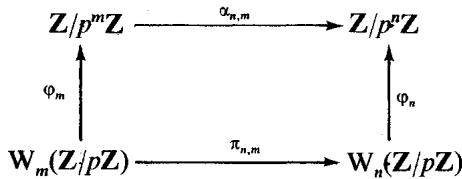
\includegraphics[keepaspectratio]{images/part001_40a15710.jpg}}

is commutative. It follows that \(\varphi = \varprojlim \varphi_n\) is an isomorphism of topological rings from \(\mathbf{W}(\mathbf{Z}/p\mathbf{Z}) = \varprojlim \mathbf{W}_n(\mathbf{Z}/p\mathbf{Z})\) onto \(\mathbf{Z}_p = \varprojlim \mathbf{Z}/p^n\mathbf{Z}\) (III, § 2, no. 12, example 3).

Let \(m\) and \(n\) be two integers \(\geqslant 1\) . By construction, one has an exact sequence of additive groups

\[
0 \longrightarrow \mathrm{W} (\mathrm{A}) \xrightarrow {\mathrm{V} ^ {m}} \mathrm{W} (\mathrm{A}) \xrightarrow {\pi_ {m}} \mathrm{W} _ {m} (\mathrm{A}) \longrightarrow 0.\tag{E}
\]

Passing to quotients, the endomorphism \(V^{n}\) of the additive group of W(A) defines a homomorphism \(V_{m}^{n}\) from the additive group of \(W_{m}(A)\) to that of \(W_{m+n}(A)\) . In other words, one has a commutative diagram

\pandocbounded{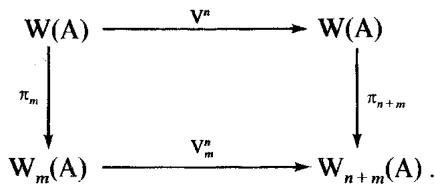
\includegraphics[keepaspectratio]{images/part001_7fe9268c.jpg}}

Passing to quotients, one deduces from the exact sequence (E) an exact sequence

\[
0 \longrightarrow \mathrm{W} _ {m} (\mathrm{A}) \xrightarrow {\mathrm{V} _ {m} ^ {n}} \mathrm{W} _ {n + m} (\mathrm{A}) \xrightarrow {\pi_ {n , n + m}} \mathrm{W} _ {n} (\mathrm{A}) \longrightarrow 0.\tag{E'}
\]

We have

\[
\mathrm{V} _ {m} ^ {n} [ a _ {0}, \dots , a _ {m - 1} ] = [ \underbrace {0 , \dots , 0} _ {n \text {   times }}, a _ {0}, \dots , a _ {m - 1} ],\tag{45}
\]

for every element \([a_0, \ldots, a_{m-1}]\) of \(\mathbf{W}_m(\mathbf{A})\) .

By prop. 3, c) of no. 5, one has FV \(^{m+1}\) (a) = p.V \(^{m}\) (a) for all a in W(A) and we consequently have F(V \(_{m+1}\) (A)) ⊂ V \(_{m}\) (A). By induction on n, it follows that F \(^{n}\) maps V \(_{n+m}\) (A) into V \(_{m}\) (A), and therefore defines, by passing to quotients, a ring homomorphism F \(^{n}\) :W \(_{n+m}\) (A) → W \(_{m}\) (A). By construction, we have a commutative diagram

\pandocbounded{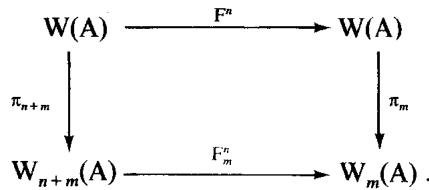
\includegraphics[keepaspectratio]{images/part001_14e9ec0a.jpg}}

Recall (no. 3) that the polynomial \(\mathbf{F}_i\) belongs to \(\mathbf{Z}[\mathbf{X}_0, \ldots, \mathbf{X}_{i+1}]\) for every integer \(i \geqslant 0\) ; the homomorphism \(\mathbf{F}_m^1\) from \(\mathbf{W}_{m+1}(\mathbf{A})\) to \(\mathbf{W}_m(\mathbf{A})\) is therefore made explicit as follows:

\[
\mathrm{F} _ {m} ^ {1} \left[ a _ {0}, \dots , a _ {m} \right] = \left[ \mathrm{F} _ {i} \left(a _ {0}, \dots , a _ {i + 1}\right) \right] _ {0 \leqslant i <   m}.\tag{46}
\]

Let \(\boldsymbol{a} \in \mathrm{W}_{m}(\mathbf{A})\) , \(\boldsymbol{a}' \in \mathrm{W}_{m}(\mathbf{A})\) and \(\boldsymbol{b} \in \mathrm{W}_{m+1}(\mathbf{A})\). The following formulas result by passing to quotients from Prop. 3 of No. 5:

\begin{enumerate}
\def\labelenumi{(\arabic{enumi})}
\setcounter{enumi}{46}
\tightlist
\item
\end{enumerate}

\[
\mathrm{F} _ {m} ^ {1} \left(\mathrm{V} _ {m} ^ {1} (\boldsymbol {a})\right) = p. \boldsymbol {a}\tag{48}
\]

\[
\mathrm{V} _ {m} ^ {1} (a \times \mathrm{F} _ {m} ^ {1} (b)) = \mathrm{V} _ {m} ^ {1} (a) \times b\tag{49}
\]

\[
\mathrm{V} _ {m} ^ {1} (a) \times \mathrm{V} _ {m} ^ {1} (a ^ {\prime}) = p. \mathrm{V} _ {m} ^ {1} (a \times a ^ {\prime})\tag{50}
\]

\[
\mathrm{V} _ {m} ^ {1} (\mathrm{F} _ {m} ^ {1} (b)) = \mu_ {m + 1} \times b
\]

\((\text{with } \boldsymbol{\mu}_{m+1} = [0, 1, 0, ..., 0]).\)

\subsection{The ring of Witt vectors with coefficients in a ring of characteristic p}

PROPOSITION 5. --- Let A be a ring of characteristic p (A, V, p. 2). For any elements a and b of W(A), and positive integers m and n, if \(\boldsymbol{a} = (a_{n})_{n \in \mathbb{N}}\) ,

\begin{enumerate}
\def\labelenumi{(\arabic{enumi})}
\setcounter{enumi}{50}
\tightlist
\item
\end{enumerate}

\[
\mathrm{F} (\boldsymbol {a}) = (a _ {n} ^ {p}) _ {n \in \mathbf {N}}\tag{52}
\]

\[
p. \boldsymbol {a} = \operatorname{VF} (\boldsymbol {a}) = \operatorname{FV} (\boldsymbol {a}) = (0, a _ {0} ^ {p}, a _ {1} ^ {p}, \dots)\tag{53}
\]

\[
\mathrm{V} ^ {m} (a) \times \mathrm{V} ^ {n} (b) = \mathrm{V} ^ {m + n} (\mathrm{F} ^ {n} (a) \times \mathrm{F} ^ {m} (b)).
\]

Formula (51) follows from Example 4 of No. 3. From this we immediately deduce the equality

\[
\operatorname{VF} (\boldsymbol {a}) = \operatorname{FV} (\boldsymbol {a}) = (0, a _ {0} ^ {p}, a _ {1} ^ {p}, \dots),
\]

and the equality \(p\) . \(a = \text{FV}(a)\) was proved (no. 5, prop. 3), whence (52).

Let us prove (53). By formula (37) (where we substitute \(V^n(\boldsymbol{b})\) for \(\boldsymbol{b}\) ), we have

\[
\mathrm{V} ^ {m} (\boldsymbol {a}) \times \mathrm{V} ^ {n} (\boldsymbol {b}) = \mathrm{V} ^ {m} \left(\boldsymbol {a} \times \mathrm{F} ^ {m} \left(\mathrm{V} ^ {n} (\boldsymbol {b})\right)\right).\tag{54}
\]

From formula (37), we also deduce

\[
\mathrm{V} ^ {n} \left(\mathrm{F} ^ {m} (\boldsymbol {b})\right) \times \boldsymbol {a} = \mathrm{V} ^ {n} \left(\mathrm{F} ^ {m} (\boldsymbol {b}) \times \mathrm{F} ^ {n} (\boldsymbol {a})\right).\tag{55}
\]

Formula (53) then follows from (54) and (55) and the relation \(F^{m} \circ V^{n} = V^{n} \circ F^{m}\) , itself a consequence of (51).

COROLLARY. --- If m and n are two positive integers, we have

\[
\mathrm{V} _ {m} (\mathrm{A}) \times \mathrm{V} _ {n} (\mathrm{A}) \subset \mathrm{V} _ {m + n} (\mathrm{A}).
\]

This follows from formula (53), since \(V_{m}(A)\) is the image of \(V^{m}:W(A)\to W(A)\) .

PROPOSITION 6.---Let A be a ring.

\begin{enumerate}
\def\labelenumi{\alph{enumi})}
\item
  For every integer \(k \geqslant 1\) , one has \((\mathrm{V}_1(\mathrm{A}))^k = p^{k-1} \cdot \mathrm{V}_1(\mathrm{A})\) .
\item
  Suppose that A is a ring of characteristic p. On the ring W(A), the V₁(A)-adic topology and the p-adic topology coincide, and they are finer than the product topology ℰ (cf. no. 6). The ring W(A) is separated and complete for the p-adic topology.
\end{enumerate}

Let us prove \(a\) ) by induction on \(k\) . The case \(k = 1\) is evident. Suppose \(k \geqslant 2\) . By the induction hypothesis, we have \(\mathrm{V}_{1}(\mathrm{A})^{k-1} = p^{k-2} \cdot \mathrm{V}_{1}(\mathrm{A})\) and consequently \(\mathrm{V}_{1}(\mathrm{A})^{k} = p^{k-2} \cdot (\mathrm{V}_{1}(\mathrm{A}))^{2}\) . But it follows from prop. 3, \(d\) ), formula (31), of no. 5 that one has \((\mathrm{V}_{1}(\mathrm{A}))^{2} = p \cdot \mathrm{V}_{1}(\mathrm{A})\) , whence \(a\) ).

Suppose now that A has characteristic p. Since one has

\[
p. \mathrm{W} (\mathrm{A}) = \mathrm{VF} (\mathrm{W} (\mathrm{A})) \subset \mathrm{V} _ {1} (\mathrm{A}) \quad (\text { formula (52) }),
\]

one deduces from \(a\) ) the inclusions \(p^{k} \cdot \mathbf{W}(\mathbf{A}) \subset (\mathbf{V}_{1}(\mathbf{A}))^{k} \subset p^{k-1} \cdot \mathbf{W}(\mathbf{A})\) , and from the corollary to prop. 5 the inclusion \((\mathbf{V}_{1}(\mathbf{A}))^{k} \subset \mathbf{V}_{k}(\mathbf{A})\) , for every integer \(k \geqslant 1\) . The first assertion of \(b\) ) follows from this.

Let \(k\) be an integer \(\geqslant 1\) . By formula (52), the ideal \(p^{k}\) . W(A) of W(A) is the set of elements \(\boldsymbol{a} = (a_{n})_{n \in \mathbf{N}}\) of W(A) such that one has \(a_{n} = 0\) for \(n < k\) and \(a_{n} \in A^{p^{k}}\) for \(n \geqslant k\) . It is therefore closed for the topology \(\mathcal{G}\) . Since W(A) is separated and complete for the topology \(\mathcal{G}\) and the ideals \(p^{k}\) . W(A) of W(A), for \(k \geqslant 1\) , form a neighborhood base of 0 in W(A) for the \(p\)-adic topology, the ring W(A) is separated and complete for the \(p\)-adic topology (TG, III, p. 26, cor. 1 to prop. 10).

PROPOSITION 7. --- Let A be a perfect ring of characteristic p.

\begin{enumerate}
\def\labelenumi{\alph{enumi})}
\item
  For every element \(\boldsymbol{a} = (a_{n})_{n \in \mathbb{N}}\) of W(A), the series with general term \(p^{n}\tau(a_{n}^{p^{-n}})\) is convergent in W(A), with sum a.
\item
  On \(\mathbf{W}(\mathbf{A})\) , the \(\mathbf{V}_1(\mathbf{A})\)-adic topology, the \(p\)-adic topology and the topology \(\mathcal{C}\) coincide. More precisely, we have \(\mathbf{V}_n(\mathbf{A}) = p^n\) . \(\mathbf{W}(\mathbf{A}) = (\mathbf{V}_1(\mathbf{A}))^n\) for every integer \(n \geqslant 0\) . In particular \(\Phi_0\) defines an isomorphism from \(\mathbf{W}(\mathbf{A})/p\) . \(\mathbf{W}(\mathbf{A})\) onto \(\mathbf{A}\) .
\end{enumerate}

By definition (A, V, p. 5), the map \(a \mapsto a^{p}\) is an automorphism of the ring A. By prop. 5, F is therefore an automorphism of the ring W(A), and one has, for every \(n \in \mathbf{N}\) ,

\[
p ^ {n}. \mathrm{W} (\mathrm{A}) = \mathrm{V} ^ {n} \mathrm{F} ^ {n} (\mathrm{W} (\mathrm{A})) = \mathrm{V} ^ {n} (\mathrm{W} (\mathrm{A})) = \mathrm{V} _ {n} (\mathrm{A}).
\]

In particular, we have \((\mathbf{V}_1(\mathbf{A}))^n = (p.\mathbf{W}(\mathbf{A}))^n = p^n.\mathbf{W}(\mathbf{A})\) . The assertion \(b)\) follows from that. By prop. 5, we have

\[
p ^ {n} \cdot \tau (a _ {n} ^ {p ^ {- n}}) = \mathrm{V} ^ {n} \mathrm{F} ^ {n} \tau (a _ {n} ^ {p ^ {- n}}) = \mathrm{V} ^ {n} \tau (a _ {n}),
\]

and assertion a) follows from prop. 4 of no. 6.

PROPOSITION 8. — Let A be a field of characteristic p. The ring W(A) is a local integral domain, separated and complete, with maximal ideal V₁(A) and residue field isomorphic to A. If the field A is perfect, the ring W(A) is a discrete valuation ring, and its maximal ideal is p.W(A).

The homomorphism \(\Phi_{0}\) defines an isomorphism from W(A)/V \(_{1}\) (A) onto A (no. 7, example 1). The ideal V \(_{1}\) (A) of W(A) is therefore maximal. Since the ring W(A) is separated and complete for the topology V \(_{1}\) (A)-adic (prop. 6, b)), it is a local ring, with maximal ideal V \(_{1}\) (A) (III, § 2, no. 13, prop. 19).

Let \(\pmb{a}\) and \(\pmb{b}\) be two nonzero elements of \(\mathbf{W}(\mathbf{A})\) . There exist integers \(m \geqslant 0\) and \(n \geqslant 0\) , and elements \(\pmb{a}' = (a_n')_{n \in \mathbb{N}}\) and \(\pmb{b}' = (b_n')_{n \in \mathbb{N}}\) of \(\mathbf{W}(\mathbf{A})\) such that \(\pmb{a} = \mathbf{V}^m(\pmb{a}')\) , \(\pmb{b} = \mathbf{V}^n(\pmb{b}')\) and such that the elements \(a_0'\) and \(b_0'\) of \(\mathbf{A}\) are nonzero. Then the component of index \(m + n\) of \(\pmb{a} \times \pmb{b}\) is equal to the component of index 0 of \(\mathbf{F}^n(\pmb{a}') \times \mathbf{F}^m(\pmb{b}')\) (formula (53)), that is, to \(a_0'^{p^n} b_0'^{p^m}\) (formula (51) and no. 3, example 2). Consequently \(\pmb{a} \times \pmb{b}\) is nonzero and \(\mathbf{W}(\mathbf{A})\) is integral.

If the field A is perfect, the maximal ideal \(V_{1}(A)\) of \(W(A)\) is equal to p.\(W(A)\)

(prop. 7, b)) and consequently W(A) is a discrete valuation ring (VI, § 3, no. 6, prop. 9, c)).

Remarks. --- 1) Let A be a field of characteristic p. One can show that the ring W(A) is Noetherian if and only if A is perfect (p. 43, exerc. 9).

\begin{enumerate}
\def\labelenumi{\arabic{enumi})}
\setcounter{enumi}{1}
\tightlist
\item
  Let A be a ring of characteristic p. By prop. 5, we have the formulas
\end{enumerate}

\[
\mathrm{F} _ {m} ^ {n} [ a _ {0}, \dots , a _ {n + m - 1} ] = [ a _ {0} ^ {p ^ {n}}, \dots , a _ {m - 1} ^ {p ^ {n}} ]
\]

\[
p ^ {n} \cdot [ a _ {0}, \dots , a _ {n + m - 1} ] = [ \underbrace {0 , \dots , 0} _ {n \text {   times }}, a _ {0} ^ {p ^ {n}}, \dots , a _ {m - 1} ^ {p ^ {n}} ]
\]

for every Witt vector \([a_0, \dots, a_{n+m-1}]\) of length \(n + m\) .

In fact, the map \(F:W(A)\to W(A)\) allows one, by passing to quotients by \(V_{m}(A)\) , to define a map \(\overline{F}_{m}:W_{m}(A)\to W_{m}(A)\) . We have the formula

\[
\overline {{{{\mathrm{F}}}}} _ {m} \left[ a _ {0}, \dots , a _ {m - 1} \right] = \left[ a _ {0} ^ {p}, \dots , a _ {m - 1} ^ {p} \right].
\]

The maps \(V_{m}^{1} \circ \overline{F}_{m}\) and \(\overline{F}_{m+1} \circ V_{m}^{1}\) from \(W_{m}(A)\) to \(W_{m+1}(A)\) are equal and are deduced, by passing to the quotient, from multiplication by p in \(W_{m+1}(A)\) .

\section{COHEN RINGS}

Throughout this section, p denotes a prime number.

\subsection{\texorpdfstring{\(p\) -rings}{p-rings}}

DEFINITION 1. --- A ring C is said to be a p-ring if the ideal pC of C is maximal, and if C is separated and complete for the pC-adic topology.

Let C be a ring; if \(p1_{C}\) is nilpotent and if the ideal pC of C is maximal, C is a p-ring, for the pC-adic topology of C is discrete. In particular, every field of characteristic p is a p-ring.

PROPOSITION 1. --- Let C be a p-ring.

\begin{enumerate}
\def\labelenumi{\alph{enumi})}
\item
  The ring C is local, with maximal ideal pC.
\item
  Suppose that \(p1_{\mathbb{C}}\) is nilpotent. Let \(d\) be the smallest positive integer such that \(p^{d}1_{\mathbb{C}} = 0\) . The ideals of \(\mathbb{C}\) are of the form \(p^{k}\mathbb{C}\) with \(0 \leqslant k \leqslant d\) and one has \(p^{k}\mathbb{C} \neq p^{l}\mathbb{C}\) when \(k\) and \(l\) are two distinct integers satisfying \(0 \leqslant k \leqslant d, 0 \leqslant l \leqslant d\) . The \(\mathbb{C}\) -module \(\mathbb{C}\) is of length \(d\) .
\item
  Suppose that \(p1_{\mathbb{C}}\) is not nilpotent. Then C is a discrete valuation ring whose residue field is of characteristic \(p\) , and whose field of fractions is of characteristic 0. The ideals of the form \(p^{n}\mathbf{C}\) , with \(n \in \mathbf{N}\) , are pairwise distinct; they form all the nonzero ideals of C. The C-module C is not of finite length.
\end{enumerate}

The assertion \(a)\) follows from prop. 19 of III, § 2, no. 13.

We have \(\bigcap_{n\geqslant 0}p^{n}\mathbf{C} = \{0\}\) by hypothesis. Let \(x\neq 0\) in \(\mathbf{C}\) ; there exists an integer \(n\geqslant 0\) such that \(x\in p^n\mathbf{C}, x\notin p^{n + 1}\mathbf{C}\) ; there therefore exists an element \(y\) of \(\mathbf{C}\) such that \(x = p^n y\) ; since \(y\) does not belong to \(p\mathbf{C}\) , \(y\) is invertible.

Suppose that \(p1_{\mathbb{C}}\) is not nilpotent. If \(x\) and \(x'\) are two nonzero elements of C, there exist two integers \(n \geqslant 0\) , \(n' \geqslant 0\) and two invertible elements \(y\) , \(y'\) of C such that \(x = p^n y\) , \(x' = p^{n'} y'\) . Then one has \(xx' = p^{n+n'} yy' \neq 0\) , hence C is an integral domain. Since C is a local ring, but is not a field, and the maximal ideal \(m_{\mathbb{C}} = p\mathbb{C}\) of C is principal, C is a discrete valuation ring (VI, § 3, no. 6, prop. 9). The nonzero ideals of C are then of the form \(p^n\mathbb{C}\) by loc. cit., prop. 8, and are pairwise distinct. In particular, the ring C is not Artinian, hence the C-module C is not of finite length. The residue field C/pC of C is of characteristic \(p\) . Let \(q\) be the characteristic of the field of fractions of C. We have \(p1_{\mathbb{C}} \neq 0\) , whence \(p \neq q\) . Moreover, if \(q\) were nonzero, we would have \(q1_{\mathbb{C}} = 0\) , hence C/pC would be of characteristic \(q \neq p\) , which is absurd. This proves \(c\) ).

Suppose that \(p1_{C}\) is nilpotent. Let \(d\) be the smallest positive integer such that \(p^{d}1_{C} = 0\) . We have a sequence of ideals

\[
\mathrm{C} \supset p \mathrm{C} \supset p ^ {2} \mathrm{C} \supset \dots \supset p ^ {d - 1} \mathrm{C} \supset p ^ {d} \mathrm{C} = \{0 \}.\tag{E}
\]

If \(k\) is an integer such that \(0 \leqslant k < d\) and \(p^k\mathbf{C} = p^{k+1}\mathbf{C}\) , then we deduce

\[
p ^ {d - k - 1} p ^ {k} \mathrm{C} = p ^ {d - k - 1} p ^ {k + 1} \mathrm{C} = \{0 \}
\]

contrary to the hypothesis \(p^{d-1}1_{\mathbf{C}} \neq 0\) . Hence the elements of the sequence (E) are pairwise distinct. Let \(\mathfrak{a}\) be an ideal of C and let \(k\) be the smallest positive integer such that \(\mathfrak{a} \supset p^k\mathbf{C}\) . Let \(x\) be a nonzero element of \(\mathfrak{a}\) ; we have seen that \(x\) is of the form \(p^m u\) with \(m \geqslant 0\) and \(u\) is invertible in C. We therefore have \(p^m\mathbf{C} \subset \mathfrak{a}\) , whence \(m \geqslant k\) , and finally \(x \in p^k\mathbf{C}\) . In conclusion, we have \(\mathfrak{a} = p^k\mathbf{C}\) . The sequence (E) is then a Jordan-Hölder sequence of the C-module C, which is of length \(d\) .

COROLLARY 1. --- If the p-ring C is an integral domain, it is a discrete valuation ring, or a field of characteristic p.

Suppose C is integral. If \(p1_{\mathbf{C}}\) is nilpotent, we have \(p1_{\mathbf{C}} = 0\) , and \(\{0\}\) is a maximal ideal of C, hence C is a field of characteristic \(p\) . If \(p1_{\mathbf{C}}\) is not nilpotent, then C is a discrete valuation ring by prop. 1, c).

COROLLARY 2. --- Let C be a p-ring and a an ideal of C distinct from C. The ring C/a is a p-ring.

We may assume \(\mathfrak{a} \neq \{0\}\) . There then exists an integer \(i \geqslant 1\) such that \(\mathfrak{a} = p^i\mathrm{C}\) ; the ideal \(p\mathrm{C} / \mathfrak{a}\) of \(\mathrm{C} / \mathfrak{a}\) is maximal and we have \(p^i1_{\mathrm{C} / \mathfrak{a}} = 0\) , hence \(\mathrm{C} / \mathfrak{a}\) is a \(p\) -ring.

Let C be a \(p\) -ring. We call the length of C, and denote by \(l(\mathbf{C})\) , the least upper bound in \(\overline{\mathbf{R}}\) of the set of integers \(n \geqslant 1\) such that \(p^{n-1}1_{\mathbf{C}} \neq 0\) . When \(l(\mathbf{C})\) is finite, it is the length of the C-module C, and when \(l(\mathbf{C})\) is equal to \(+\infty\) , the C-module C is not of finite length (prop. 1).

Examples. --- 1) For every integer \(n \geqslant 1\) , the ring \(\mathbf{Z}/p^{n}\mathbf{Z}\) is a \(p\) -ring of length \(n\) . The ring \(\mathbf{Z}_{p}\) of \(p\) -adic integers is a \(p\) -ring of infinite length.

\begin{enumerate}
\def\labelenumi{\arabic{enumi})}
\setcounter{enumi}{1}
\tightlist
\item
  Let K be a perfect field of characteristic p. By prop. 8 of § 1, no. 8, the ring W(K) of Witt vectors is a p-ring of infinite length. The map \((a_{n})_{n\in\mathbf{N}} \mapsto a_{0}\) induces by passage to the quotient an isomorphism of W(K)/pW(K) onto the field K (loc. cit., prop. 7). For every integer \(n \geqslant 1\) , the ring
\end{enumerate}

\[
\mathrm{W} _ {n} (\mathrm{K}) = \mathrm{W} (\mathrm{K}) / p ^ {n} \mathrm{W} (\mathrm{K})
\]

is a p-ring of length n.

PROPOSITION 2. --- Let C and C' be two p-rings and let \(u\) be a homomorphism from C to C'. Let \(v\) be the homomorphism from \(\kappa_{\mathbf{C}} = \mathbf{C} / p\mathbf{C}\) to \(\kappa_{\mathbf{C}'} = \mathbf{C}' / p\mathbf{C}'\) induced by u by passage to the quotients.

\begin{enumerate}
\def\labelenumi{\alph{enumi})}
\item
  We have \(l(\mathbf{C}) \geqslant l(\mathbf{C}')\) and u is injective if and only if \(l(\mathbf{C}) = l(\mathbf{C}')\) .
\item
  For u to be surjective, it is necessary and sufficient that v be an isomorphism.
\item
  For u to be an isomorphism, it is necessary and sufficient that v be an isomorphism and that we have \(l(\mathbf{C}) = l(\mathbf{C}')\) .
\end{enumerate}

Let \(n \geqslant 1\) be an integer. One has \(u(p^{n-1}1_{\mathbf{C}}) = p^{n-1}1_{\mathbf{C}'}\) , hence the relation \(p^{n-1}1_{\mathbf{C}'} \neq 0\) implies \(p^{n-1}1_{\mathbf{C}} \neq 0\) and is equivalent to it if \(u\) is injective. We therefore have \(l(\mathbf{C}') \leqslant l(\mathbf{C})\) with equality if \(u\) is injective. If \(u\) is not injective, there exists an integer \(i < l(\mathbf{C})\) such that the kernel of \(u\) is the ideal \(p^i\mathbf{C}\) of \(\mathbf{C}\) ; we then have \(p^i1_{\mathbf{C}'} = 0\) , whence \(l(\mathbf{C}') \leqslant i\) . This proves \(a\) ).

Since \(\kappa_{\mathrm{C}}\) and \(\kappa_{\mathrm{C}'}\) are fields, the homomorphism \(v\) is injective. If \(u\) is surjective, so is \(v\) , which is therefore an isomorphism. Conversely, suppose \(v\) is surjective. Then for every integer \(n \geqslant 0\) , the map \(v_{n}: p^{n}\mathrm{C}/p^{n+1}\mathrm{C} \to p^{n}\mathrm{C}'/p^{n+1}\mathrm{C}'\) derived from \(u\) is surjective. Since C is complete for the \(p\mathrm{C}\)-adic filtration and \(\mathbf{C}'\) separated for the \(p\mathbf{C}'\)-adic filtration, \(u\) is surjective by Cor. 2 of Th. 1 of III, § 2, No. 8. This proves \(b\) ).

Finally, c) follows from a) and b).

PROPOSITION 3. --- Let \((\mathbf{C}_{n}, \pi_{n,m})\) be a projective system of rings relative to the index set N. We assume that \(\mathbf{C}_{n}\) is a p-ring for all \(n \in \mathbf{N}\) and that the homomorphisms \(\pi_{n,m}\) are surjective. Then \(C = \varprojlim C_{n}\) is a p-ring, and for all \(n \in \mathbf{N}\) the canonical homomorphism \(\pi_{n}: C \to C_{n}\) is surjective and induces an isomorphism of \(\kappa_{C}\) onto \(\kappa_{C_{n}}\) .

As the maps \(\pi_{n,m}\) are surjective, the same holds for the maps \(\pi_n\) (E, III, p. 58, prop. 5). Let us show that C is a \(p\) -ring. Let \(d_n\) be the length of \(\mathbf{C}_n\) . By prop. 2, a), the sequence of elements \(d_n\) of \(\mathbf{N} \cup \{+\infty\}\) is increasing; if it is stationary, there exists an integer \(n_0\) such that \(\pi_{n,m}\) is an isomorphism of \(\mathbf{C}_m\) onto \(\mathbf{C}_n\) when \(n_0 \leqslant n \leqslant m\) , so that C, which is isomorphic to \(\mathbf{C}_{n_0}\) , is a \(p\) -ring.

It therefore suffices to consider the case where each \(d_{n}\) is finite, and where the sequence \((d_{n})\) tends to \(+\infty\) . Endow the ring C with the trivial filtration (III, § 2, n° 1, example 5). For \(n\in\mathbf{N}\) , let \(\mathbf{I}_{n}\) be the kernel of \(\pi_{n}\) ; set \(\mathbf{I}_{n}=\mathbf{C}\) if \(n<0\) . Let E denote the C-module C equipped with the filtration \((\mathbf{I}_{n})_{n\in\mathbf{Z}}\) . It is separated and complete, because the topology \(\mathcal{G}\) defined by the filtration \((\mathbf{I}_{n})_{n\in\mathbf{Z}}\) is the projective limit topology of the discrete topologies on the \(\mathbf{C}_{n}\) .

Let \(k\) be an integer \(\geqslant 1\) . We have \(p^{k}\mathrm{C} \subset \varprojlim (p^{k}\mathrm{C}_{n})\) (E, III, p. 55, formula (9)). Conversely, if \(x = (x_{n})_{n \in \mathbb{N}} \in \varprojlim (p^{k}\mathrm{C}_{n})\) and if one sets \(\mathrm{X}_{n} = \{y \in \mathrm{C}|\pi_{n}(p^{k}y) = x_{n}\}\) , the sequence \((\mathrm{X}_{n})_{n \in \mathbb{N}}\) is a decreasing sequence of nonempty closed affine subsets of E. Since \(\mathrm{E / I}_{n}\) is an artinian C-module, the intersection of the \(\mathrm{X}_{n}\) is nonempty (III, § 2, n° 7, prop. 7); for every \(z \in \bigcap_{n \in \mathbb{N}} \mathrm{X}_{n}\) we have \(p^{k}z = x\) . We have therefore proved that one has \(p^{k}\mathrm{C} = \varprojlim p^{k}\mathrm{C}_{n}\) .

for every integer \(k \geqslant 1\) . In particular, the ideal \(p^{k}\text{C}\) of C is closed for the topology \(\mathcal{G}\) . On C, the \(p\) -adic topology is finer than the topology \(\mathcal{G}\) because one has \(p^{d_{n}}\text{C} \subset \text{I}_{n}\) . It then follows from TG, III, p. 26, cor. 1 to prop. 10, that C is separated and complete for the \(p\text{C}\) -adic topology. Moreover, one has \(p\text{C} = \varprojlim p\text{C}_{n} = \pi_{0}^{-1}(p\text{C}_{0})\) and hence the surjective homomorphism of C/pC into \(\text{C}_{0}/p\text{C}_{0}\) deduced from \(\pi_{0}\) is an isomorphism. This shows that the ideal \(p\text{C}\) of C is maximal and consequently that C is a \(p\) -ring. The last assertion of prop. 3 follows from prop. 2, b).

\subsection{Cohen rings}

DEFINITION 2. --- Let A be a separated and complete local ring, whose residue field is of characteristic p. One calls a Cohen subring of A a subring C of A which is a p-ring such that \(\mathbf{A} = \mathfrak{m}_{\mathbf{A}} + \mathbf{C}\) (i.e. \(\mathbf{A}/\mathfrak{m}_{\mathbf{A}} = \mathbf{C}/(\mathfrak{m}_{\mathbf{A}} \cap \mathbf{C})\) ).

If C is a Cohen subring of A, the ideal \(m_{A} \cap C\) of C is maximal, hence equal to pC. The canonical map from \(\kappa_{C} = C/pC\) onto \(\kappa_{A} = A/m_{A}\) is therefore an isomorphism of fields.

Example. --- Let C be a p-ring. The ring of formal power series \(A = C[[T_{1}, \ldots, T_{n}]]\) is a Noetherian local ring, separated and complete, whose maximal ideal is generated by the sequence (p, T₁, \ldots, Tₙ). It is immediate that C is a Cohen subring of A. This applies in particular when C is equal to Zₚ, to Z/pⁿZ, or to a field of characteristic p.

THEOREM 1. — Let A be a local ring, separated and complete, whose residue field k has characteristic p. Let π be the canonical map from A onto k, and let S be a subset of A such that π induces a bijection from S onto a p-basis of k (A, V, p. 95).

\begin{enumerate}
\def\labelenumi{\alph{enumi})}
\item
  There exists a Cohen subring C of A containing S, and it is unique.
\item
  The subring C of A is closed, and the \(p\)C-adic topology on C is induced by the \(m_{A}\)-adic topology of A.
\item
  Every closed subring A' of A, containing S, and such that \(A = A' + m_{A}\) contains C.
\end{enumerate}

\begin{enumerate}
\def\labelenumi{\Alph{enumi})}
\tightlist
\item
  Special case: \(\mathfrak{m}_{\mathbf{A}}\) nilpotent
\end{enumerate}

Let \(n\) be a positive integer such that \(\mathfrak{m}_{\mathbf{A}}^{n+1}=\{0\}\) . If \(\Phi_{n}\) is the \(n\) -th Witt polynomial ( § 1, no. 1 ), the map \(u:[a_{0},..., a_{n}]\mapsto\Phi_{n}(a_{0},..., a_{n})\) is a ring homomorphism from \(\mathbf{W}_{n+1}(\mathbf{A})\) to \(\mathbf{A}\) ( § 1, no. 7 ). Let \(\mathbf{B}_{n}\) be the image of \(u\) and let \(\mathbf{C}_{n}\) be the subring of \(\mathbf{A}\) generated by \(\mathbf{B}_{n}\cup\mathbf{S}\) .

Lemma 1. --- Let A' be a subring of A containing S. For A' to contain \(\mathbf{C}_{n}\) , it is necessary and sufficient that \(A' + m_{A} = A\).

We have \(pA \subset m_A\) and \(B_n\) consists of the elements of the form \(a_0^{p^n} + pa_1^{p^{n-1}} + \cdots + p^n a_n\) with \(a_0, \ldots, a_n\) in A. Consequently, we have \(\pi(B_n) = k^{p^n}\) , whence \(\pi(C_n) = k^{p^n}[\pi(S)]\) . But since \(\pi(S)\) is a \(p\) -basis of \(k\) , one has \(k = k^{p^n}[\pi(S)]\) (A, V, p. 96), whence \(\pi(C_n) = k\) , that is, \(C_n + m_A = A\) .

Let A' be a subring of A containing S. If A' contains \(C_{n}\) , one has

\[
\mathrm{A} ^ {\prime} + \mathrm{m} _ {\mathrm{A}} \supset \mathrm{C} _ {n} + \mathrm{m} _ {\mathrm{A}} = \mathrm{A}, \quad \mathrm{whence} \quad \mathrm{A} ^ {\prime} + \mathrm{m} _ {\mathrm{A}} = \mathrm{A}.
\]

Conversely, suppose we have \(\mathbf{A}' + \mathfrak{m}_{\mathbf{A}} = \mathbf{A}\) . Let \(a_0, \ldots, a_n\) be elements of \(\mathbf{A}\) ; by hypothesis there exist elements \(a_0', \ldots, a_n'\) of \(\mathbf{A}'\) such that \(a_i \equiv a_i'\) mod. \(\mathfrak{m}_{\mathbf{A}}\) for \(0 \leqslant i \leqslant n\) . By prop. 1 of § 1, no. 1 and the hypothesis \(\mathfrak{m}_{\mathbf{A}}^{n+1} = \{0\}\) , one therefore has \(\Phi_n(a_0, \ldots, a_n) = \Phi_n(a_0', \ldots, a_n') \in \mathbf{A}'\) , whence \(\mathbf{B}_n \subset \mathbf{A}'\) . Since \(\mathbf{C}_n\) is the ring generated by \(\mathbf{B}_n \cup \mathbf{S}\) , one has \(\mathbf{C}_n \subset \mathbf{A}'\) .

In the set S of subrings A' of A containing S and such that \(A' + m_{A} = A\) there exists, by lemma 1, a smallest element C, and one has \(C_{n} = C\) for every integer \(n \geqslant 0\) such that \(m_{A}^{n+1} = \{0\}\) .

We have \(C + m_A = A\) by construction and \(p1_C\) is nilpotent. One obviously has \(pC \subset C \cap m_A\) and lemma 2 below therefore shows that \(pC\) is a maximal ideal of \(C\) and consequently that \(C\) is a Cohen subring of \(A\) .

Lemma 2. --- One has \(C \cap m_{A} \subset pC\).

Let us choose an integer \(m \geqslant 1\) such that \(\mathfrak{m}_{\mathbf{A}}^{m} = \{0\}\) , whence \(\mathbf{C} = \mathbf{C}_{m} = \mathbf{C}_{m-1}\) . Let \(\Lambda\) be the part of \(\mathbf{N}^{(\mathbf{S})}\) consisting of families with finite support of integers \((\alpha_{s})_{s \in \mathbf{S}}\) satisfying \(0 \leqslant \alpha_{s} < p^{m}\) for every \(s \in \mathbf{S}\) . Since \(\mathbf{B}_{m}\) contains \(s^{p^{m}} = \Phi_{m}(s, 0, ..., 0)\) for every \(s \in \mathbf{S}\) , the monomials \(Z_{\alpha} = \prod_{s \in \mathbf{S}} s^{\alpha_{s}}\) , where \(\alpha\) ranges over \(\Lambda\) , generate \(\mathbf{C}_{m}\) as a \(\mathbf{B}_{m}\) -module. Moreover, by the formula

\[
\Phi_ {m} (a _ {0}, \dots , a _ {m}) = a _ {0} ^ {p ^ {m}} + p \Phi_ {m - 1} (a _ {1}, \dots , a _ {m}),
\]

every element of \(B_{m}\) is of the form \(a^{p^{m}} + pb\) with \(a \in A\) and \(b \in B_{m-1}\) . Consequently every element of \(C = C_{m}\) is of the form

\[
x = \sum_ {\alpha \in \Lambda} c _ {\alpha} ^ {p ^ {m}} Z _ {\alpha} + p y\tag{1}
\]

with \(c_{\alpha} \in \mathbf{A}\) for every \(\alpha \in \Lambda\) , and \(y \in \mathbf{C}_{m-1} = \mathbf{C}\) . If \(x\) belongs to \(\mathbf{C} \cap \mathfrak{m}_{\mathbf{A}}\) , one has \(\pi(x) = 0\) , whence \(\sum_{\alpha \in \Lambda} \pi(c_{\alpha})^{p^m} \pi(Z_{\alpha}) = 0\) . Since \(\pi(\mathbf{S})\) is a \(p\) -basis of \(k\) , one has \(\pi(c_{\alpha}) = 0\) for every \(\alpha \in \Lambda\) according to A, V, p. 96. We then have \(c_{\alpha} \in \mathfrak{m}_{\mathbf{A}}\) , whence \(c_{\alpha}^m = 0\) and a fortiori \(c_{\alpha}^{p^m} = 0\) . By (1), we have \(x = py\) , whence lemma 2.

We have \(p^m\mathbf{C} = \mathfrak{m}_{\mathbf{A}}^m = \{0\}\) for \(m\) sufficiently large, and assertion \(b)\) is therefore trivial. Assertion \(c)\) follows from lemma 1. If \(\mathbf{C}'\) is a Cohen subring of A containing S, we have \(\mathbf{C}' \supset \mathbf{C}\) by lemma 1. But since the inclusion of C in \(\mathbf{C}'\) induces an isomorphism of \(\kappa_{\mathbf{C}}\) onto \(\kappa_{\mathbf{C}'}\) , one has \(\mathbf{C} = \mathbf{C}'\) (no. 1, prop. 2, b)), and this completes the proof of \(a\) ).

\noindent\textbf{B) General case.}\par

For every integer \(n \geqslant 0\) , denote by \(\mathbf{A}_n\) the local ring \(\mathbf{A}/\mathfrak{m}_{\mathbf{A}}^{n+1}\) , \(\mathfrak{m}_n = \mathfrak{m}_{\mathbf{A}}/\mathfrak{m}_{\mathbf{A}}^{n+1}\) its maximal ideal, and \(\pi_n\) the canonical homomorphism from A onto \(\mathbf{A}_n\) . By A), there exists a unique Cohen subring \(\mathbf{C}_n\) of \(\mathbf{A}_n\) containing \(\pi_n(\mathbf{S})\) . When \(0 \leqslant n \leqslant m\) , denote by \(\pi_{n,m}\) the canonical homomorphism from \(\mathbf{A}_m\) onto \(\mathbf{A}_n\) . By cor. 2 of prop. 1 of no. 1, \(\pi_{n,m}(\mathbf{C}_m)\) is a \(p\) -ring; we have \(\pi_{n,m}(\mathbf{C}_m) + \mathfrak{m}_n = \mathbf{A}_n\) , hence \(\pi_{n,m}(\mathbf{C}_m)\) is equal to the Cohen subring \(\mathbf{C}_n\) of \(\mathbf{A}_n\) . By prop. 3 of no. 1, the subring \(\varprojlim \mathbf{C}_n\) of \(\varprojlim \mathbf{A}_n\) is a \(p\) -ring. Set \(\mathbf{C} = \bigcap_{n \in \mathbb{N}} \pi_n^{-1}(\mathbf{C}_n)\) . Since C is the inverse image of \(\varprojlim \mathbf{C}_n\) under the isomorphism \(a \mapsto (\pi_n(a))_{n \in \mathbb{N}}\) from A onto \(\varprojlim \mathbf{A}_n\) , it is a closed subring of A, and a \(p\) -ring. We have \(\pi_n(\mathbf{C}) = \mathbf{C}_n\) for every \(n \in \mathbb{N}\) (no. 1, prop. 3), and in particular \(\pi_0(\mathbf{C}) = \mathbf{A}_0\) , that is, \(\pi(\mathbf{C}) = k\) . Hence C is a Cohen subring of A.

For every integer \(n \geqslant 0\) , set \(J_{n} = C \cap m_{A}^{n}\) . Since the local ring A is separated, we have \(\bigcap_{n \in \mathbb{N}} J_{n} = \{0\}\) , and in view of the structure of ideals of a \(p\) -ring (no. 1, prop. 1), every ideal of C of the form \(p^{k}C\) contains one of the \(J_{n}\) . Conversely, \(J_{n}\) contains \(p^{n}C\) . Hence, the \(pC\) -adic topology of C is induced by the \(m_{A}\) -adic topology of A. This proves \(b\) ).

Let A' be a closed subring of A, containing S and such that \(A' + m_{A} = A\). Since A' is closed, we have A' = \(\bigcap_{n\in\mathbb{N}}\pi_n^{-1}(\pi_n(A'))\) . We have \(\pi_n(A') \supset \pi_n(S)\) and \(\pi_n(A') + m_n = A_n\) , whence \(\pi_n(A') \supset C_n\) according to what was seen in A). Finally, we have \(\pi_n^{-1}(\pi_n(A')) \supset \pi_n^{-1}(C_n)\) , whence A' ⊃ C. This proves c). From this we deduce the uniqueness of a Cohen subring as in A).

Remark. --- Suppose that \(p1_{A}\) is not nilpotent (this occurs in particular when A is an integral domain whose field of fractions has characteristic 0). Then C is a discrete valuation ring whose field of fractions has characteristic 0.

\subsection{Existence and uniqueness of p-rings}

PROPOSITION 4. --- Let C and C' be two p-rings such that \(l(\mathbf{C}) \geqslant l(\mathbf{C}')\) , and let \(\pi\) (resp. \(\pi'\) ) be the canonical homomorphism from C (resp. C') onto \(\kappa_{\mathbf{C}}\) (resp. \(\kappa_{\mathbf{C}'}\) ). Let \((x_{\lambda})_{\lambda \in \Lambda}\) (resp. \((x_{\lambda}')_{\lambda \in \Lambda}\) ) be a family of elements of C (resp. C') whose images under \(\pi\) (resp. \(\pi'\) ) form a p-basis of \(\kappa_{\mathbf{C}}\) (resp. \(\kappa_{\mathbf{C}'}\) ). Let v be an isomorphism of \(\kappa_{\mathbf{C}}\) onto \(\kappa_{\mathbf{C}'}\) such that \(v(\pi(x_{\lambda})) = \pi'(x_{\lambda}')\) for every \(\lambda \in \Lambda\) . There then exists a unique homomorphism u from C to C' such that \(v \circ \pi = \pi' \circ u\) and \(u(x_{\lambda}) = x_{\lambda}'\) for every \(\lambda \in \Lambda\) . It is surjective. If \(l(\mathbf{C}) = l(\mathbf{C}')\) , it is an isomorphism.

Let us prove the existence of u. Let A be the subring of C × C' formed by the pairs \((x, x')\) such that \(v(\pi(x)) = \pi'(x')\) . The map \((x, x') \mapsto \pi(x)\) is a surjective ring homomorphism of A onto \(\kappa_{\mathbb{C}}\) . Its kernel m, equal to \(p\mathbb{C} \times p\mathbb{C}'\) , is therefore a maximal ideal of A. The topological subspace A of \(\mathbb{C} \times \mathbb{C}'\) is closed in \(\mathbb{C} \times \mathbb{C}'\) , hence complete, and the topology induced on A by that of \(\mathbb{C} \times \mathbb{C}'\) is the m-adic topology. Consequently A is a separated and complete local ring with maximal ideal m (III, § 2, no. 13, prop. 19). For every \(\lambda \in \Lambda\) , one has \((x_{\lambda}, x_{\lambda}') \in A\) by hypothesis; if \(\xi_{\lambda}\) is the class of \((x_{\lambda}, x_{\lambda}')\) modulo m, the family \((\xi_{\lambda})_{\lambda \in \Lambda}\) is a \(p\) -basis of the field A/m. By th. 1 of no. 2, there exists a unique Cohen subring \(\mathbb{C}''\) of A containing \((x_{\lambda}, x_{\lambda}')\) for every \(\lambda \in \Lambda\) . We have \(l(\mathbb{C}'') = l(\mathbb{C}) \geqslant l(\mathbb{C}')\) . The restriction to \(\mathbb{C}''\) of the projection of \(\mathbb{C} \times \mathbb{C}'\) onto C is a homomorphism \(h: \mathbb{C}'' \to \mathbb{C}\) which induces an isomorphism of \(\kappa_{\mathbb{C}''}\) onto \(\kappa_{\mathbb{C}}\) . By prop. 2, c) of no. 2, h is an isomorphism of \(\mathbb{C}''\) onto C. One sees in the same way that the restriction \(h'\) to \(\mathbb{C}''\) of the projection of \(\mathbb{C} \times \mathbb{C}'\) onto C' is a surjective homomorphism of \(\mathbb{C}''\) into C'. Consequently, \(\mathbb{C}''\) is the graph of a surjective homomorphism \(u = h' \circ h^{-1}\) of C onto C', and we evidently have \(v \circ \pi = \pi' \circ u\) , \(u(x_{\lambda}) = x_{\lambda}'\) for every \(\lambda \in \Lambda\) . Moreover, if \(l(\mathbb{C}) = l(\mathbb{C}')\) , u is an isomorphism.

Let us prove the uniqueness of \(u\) . Let \(u_{1}\) be a homomorphism from C to C' such that \(v \circ \pi = \pi' \circ u_{1}\) and \(u_{1}(x_{\lambda}) = x_{\lambda}'\) for every \(\lambda \in \Lambda\) , and let \(\mathbf{C}_{1}\) be the graph of \(u_{1}\) . It is immediate that \(\mathbf{C}_{1}\) is a Cohen subring of A, containing \((x_{\lambda}, x_{\lambda}')\) for every \(\lambda \in \Lambda\) , whence \(\mathbf{C}_{1} = \mathbf{C}''\) (th. 1 of no. 2) and finally \(u_{1} = u\) .

PROPOSITION 5. --- Let k be a field of characteristic p, and let n be an integer ≥ 1, or + ∞. There exists a p-ring of length n whose residue field is isomorphic to k.

The ring \(\mathbf{W}(k)\) of Witt vectors with coefficients in \(k\) is a separated and complete integral local ring, whose residue field is isomorphic to \(k\) ( \(\S\) 1, no. 8, prop. 8), and we have \(p\) . \(1_{\mathbf{W}(k)} \neq 0\) (loc. cit., formula (52)). Let C be a Cohen subring of \(\mathbf{W}(k)\) (no. 2, th. 1). Then C is a \(p\) -ring of length + \(\infty\) whose residue field is isomorphic to \(k\) , and, if \(n\) is an integer \(\geqslant 1\) , the quotient \(\mathrm{C}/p^{n}\mathrm{C}\) is a \(p\) -ring of length \(n\) whose residue field is isomorphic to \(k\) .

Remarks. --- 1) Let \(n\) be an integer \(\geqslant 1\) and S be a \(p\) -basis of \(k\) . One can show that the subring of \(\mathbf{W}_{n}(k)\) generated by \(\mathbf{W}_{n}(k^{p^{n}})\) and by the elements \([\xi, 0, ..., 0]\) ( \(\xi \in S\) ), is a \(p\) -ring of length \(n\) whose residue field is isomorphic to \(k\) (cf. p. 72, exerc. 10).

\begin{enumerate}
\def\labelenumi{\arabic{enumi})}
\setcounter{enumi}{1}
\tightlist
\item
  The reader will find in the Appendix a proof of prop. 5 which uses neither the results of § 1, nor the existence theorem for Cohen subrings (no. 2, th. 1).
\end{enumerate}

COROLLARY. --- Let C be a p-ring of finite length n. There exists a p-ring C' of infinite length such that C is isomorphic to \(C'/p^{n}C'\).

By prop. 5, there exists a \(p\) -ring \(C'\) of infinite length such that \(\kappa_{C'}\) is isomorphic to \(\kappa_{C}\) . Then \(C'/p^{n}C'=C_{n}'\) is a \(p\) -ring of length \(n\) , and the field \(\kappa_{C_{n}'}\) is isomorphic to \(\kappa_{C'}\) , hence to \(\kappa_{C}\) . By prop. 4, the rings \(C\) and \(C_{n}'\) are therefore isomorphic.

\subsection{Multiplicative representatives}

PROPOSITION 6. --- Let C be a p-ring, whose residue field k is perfect. Suppose C has finite length n (resp. infinite length). There exists a unique isomorphism \(u:W_{n}(k)\to C\) (resp. \(u:W(k)\to C\) ) which induces, by passage to quotients, the identity map of k.

Since \(W_{n}(k)\) (resp. \(W(k)\) ) is a p-ring with residue field k and of length n (resp. of infinite length) (no. 1, example 2), and since \(\varnothing\) is a p-basis of the perfect field k, prop. 6 is a special case of prop. 4 of no. 3.

THEOREM 2. --- Let A be a separated and complete local ring, k its residue field, and π the canonical homomorphism from A onto k. Suppose that k is a perfect field of characteristic p.

\begin{enumerate}
\def\labelenumi{\alph{enumi})}
\item
  There exists a unique ring homomorphism \(u: \mathbf{W}(k) \to \mathbf{A}\) such that \(\pi(u(\boldsymbol{a})) = a_0\) for \(\boldsymbol{a} = (a_n)_{n \in \mathbb{N}}\) in \(\mathbf{W}(k)\) .
\item
  The homomorphism u is continuous when W(k) is equipped with the pW(k)-adic topology, and the image of u is the unique Cohen subring of A.
\end{enumerate}

By th. 1 of no. 2, there exists a unique Cohen subring of A; denote it by C. Let u be a homomorphism from W(k) into A such that \(\pi(u(\boldsymbol{a})) = a_0\) for every \(\boldsymbol{a} = (a_n)_{n \in \mathbb{N}}\) in W(k); it is immediate that the image of u is a Cohen subring of A, hence equal to C. The existence and uniqueness of u then follow from prop. 6. The pC-adic topology of C is induced by the \(m_{A}\)-adic topology of A (no. 2, th. 1, b)), whence the continuity of u.

For a direct construction of u, see p. 70, exerc. 6.

PROPOSITION 7. --- Keep the hypotheses and notations of th. 2. There exists a unique multiplicative subset S of A such that π induces a bijection from S onto k. For an element a of A to belong to S, it is necessary and sufficient that for every n ∈ N, there exists an element \(a_{n}\) of A such that \(a = a_{n}^{p^{n}}\) . The set S is the set of elements of the form \(u(x, 0, 0, \ldots)\) .

Let us first prove the uniqueness of S. Let S be a multiplicative subset of A, such that \(\pi\) induces a bijection from S onto k. Let T be the set of elements of A which are powers \(p^{n}\) -th for every \(n \in N\) .

\begin{enumerate}
\def\labelenumi{\alph{enumi})}
\item
  We have S ⊂ T: Let \(a \in S\) and \(n \in N\) ; since the field k is perfect, there exists an element \(x_{n}\) of k such that \(x_{n}^{p^{n}} = \pi(a)\) ; since we have \(\pi(S) = k\) , there exists an element \(a_{n}\) of S such that \(x_{n} = \pi(a_{n})\) . Then one has \(\pi(a_{n}^{p^{n}}) = \pi(a)\) whence \(a_{n}^{p^{n}} = a\) since the restriction of \(\pi\) to S is injective.
\item
  The restriction of \(\pi\) to T is injective: let \(a\) and \(b\) be two elements of T such that \(\pi(a) = \pi(b)\) . Let \(n \in \mathbf{N}\) ; there exist two elements \(a_n\) and \(b_n\) of A such that \(a = a_n^{p^n}\) , \(b = b_n^{p^n}\) . Then one has \(\pi(a_n)^{p^n} = \pi(b_n)^{p^n}\) , whence \(\pi(a_n) = \pi(b_n)\) , that is, \(a_n \equiv b_n\) mod. \(\mathfrak{m}_{\mathbf{A}}\) . By lemma 1 of § 1, no. 1, we have \(a_n^{p^n} \equiv b_n^{p^n}\) mod. \(\mathfrak{m}_{\mathbf{A}}^{n+1}\) , that is, \(a \equiv b\) mod. \(\mathfrak{m}_{\mathbf{A}}^{n+1}\) . Since \(n\) is arbitrary, we have \(a = b\) .
\end{enumerate}

Properties a) and b) above, together with the formula \(\pi(S) = k\) , imply the relation \(S = T\) , whence uniqueness.

Let us now prove the existence of S. With the notations of th. 2, set \(\varphi = u \circ \tau_k\) , that is (§ 1, no. 6)

\[
\varphi (x) = u (x, 0, 0, \dots)\tag{2}
\]

for every \(x \in k\) . By prop. 4 of loc. cit., we have

\[
\varphi (1) = 1, \quad \varphi (x y) = \varphi (x) \varphi (y) \quad \text { for } \quad x, y \text {   in   } k.\tag{3}
\]

It is clear that the map \(\pi \circ \varphi\) is the identity map of \(k\) . Hence the image S of \(\varphi\) satisfies the conditions of Prop. 7.

The elements of S are often called the multiplicative (or Teichmüller) representatives of A.

Remarks. --- 1) We keep the preceding hypotheses and notation. We have

\[
\boldsymbol {a} = \sum_ {n = 0} ^ {\infty} p ^ {n} \tau_ {k} (a _ {n} ^ {p ^ {- n}}) \quad (\boldsymbol {a} = (a _ {n}) _ {n \in \mathbf {N}} \in \mathrm{W} (k))
\]

by Prop. 7 of § 1, no. 8. We therefore have

\[
u (\boldsymbol {a}) = \sum_ {n = 0} ^ {\infty} p ^ {n} \varphi (a _ {n} ^ {p ^ {- n}})\tag{4}
\]

for every \(\boldsymbol{a} = (a_n)_{n \in \mathbf{N}}\) in \(\mathrm{W}(k)\) , since \(u\) is continuous (Th. 2, b)). By formula (4), the unique Cohen subring of A consists of the elements of the form \(\sum_{n=0}^{\infty} p^n s_n\) with \(s_n \in S\) for every integer \(n \geqslant 0\) .

\begin{enumerate}
\def\labelenumi{\arabic{enumi})}
\setcounter{enumi}{1}
\tightlist
\item
  Let A be a separated and complete local ring, k its residue field, and \(\pi\) the canonical homomorphism from A onto k. One can show that there exists a multiplicative subset S of A (not unique in general) such that \(\pi\) induces a bijection from S onto k (cf. p. 72, exerc. 11).
\end{enumerate}

Examples. --- 1) Let \(k\) be a perfect field of characteristic \(p\) . The multiplicative representatives of the ring \(\mathbf{W}(k)\) are the Witt vectors \(\tau(x) = (x, 0, 0, \ldots)\) for \(x \in k\) .

\begin{enumerate}
\def\labelenumi{\arabic{enumi})}
\setcounter{enumi}{1}
\item
  Let A be an integral, separated, and complete local ring. Suppose that the residue field \(k\) of A is finite, with \(q = p^{f}\) elements, hence perfect of characteristic \(p\) . We have \(x^{q} = x\) for every \(x \in k\) , whence \(s^{q} = s\) for every multiplicative representative \(s\) . It follows that the set of multiplicative representatives consists of 0 and the \((q - 1)\)-th roots of unity in the field of fractions of A. If the field of fractions of A is locally compact, the existence of multiplicative representatives also follows from VI, § 9, no. 2, Prop. 3 (cf. also VI, § 9, exerc. 5).
\item
  More particularly, consider the case \(A = Z_{p}\) . Then the multiplicative representatives are 0 and the \((p - 1)\) -th roots of unity in the field of fractions \(Q_{p}\) of \(Z_{p}\) .
\end{enumerate}

\subsection{Structure of Noetherian and complete local rings}

Let A and C be complete Noetherian local rings, and let u be a local homomorphism from C to A, inducing by passage to quotients an isomorphism of \(\kappa_{C}\) onto \(\kappa_{A}\) . Let \((p_{1}, \ldots, p_{m})\) be a sequence generating the ideal \(m_{C}\) of C, and let \(t_{1}, \ldots, t_{n}\) be elements of \(m_{A}\) . Put \(B = C[[T_{1}, \ldots, T_{n}]]\) .

Lemma 3.--- a) There exists a unique homomorphism \(v: \mathbf{B} \to \mathbf{A}\) which extends \(u\) and maps \(\mathbf{T}_i\) to \(t_i\) for \(1 \leqslant i \leqslant n\) .

\begin{enumerate}
\def\labelenumi{\alph{enumi})}
\setcounter{enumi}{1}
\item
  For v to be surjective, it is necessary and sufficient that the sequence \((u(p_{1}), \ldots, u(p_{m}), t_{1}, \ldots, t_{n})\) generates the ideal \(m_{A}\) of A, or equivalently that the classes of these elements modulo \(m_{A}^{2}\) generate \(m_{A}/m_{A}^{2}\) as a vector space over the field \(k_{A}\) .
\item
  For \(v\) to make A a finite B-algebra, it is necessary and sufficient that the sequence \((u(p_1), \ldots, u(p_m), t_1, \ldots, t_n)\) generate an ideal of definition for the \(\mathfrak{m}_{\mathbf{A}}\)-adic topology of A.
\end{enumerate}

Let n denote the ideal of the ring B generated by \(T_{1}, \ldots, T_{n}\) . Every homomorphism v from B to A which extends u and such that \(v(T_{i}) = t_{i}\) maps n into \(m_{A}\) , hence is continuous when B is equipped with the n-adic topology. The existence and uniqueness of v then follow from A, IV, p. 26, prop. 4.

The ring \(B = C[[T_{1}, \ldots, T_{n}]]\) is a complete Noetherian local ring (III, § 2, n° 10, cor. 6 of th. 2 and n° 6, prop. 6), whose maximal ideal \(m_{B}\) is generated by \(p_{1}, \ldots, p_{m}, T_{1}, \ldots, T_{n}\) . We therefore have \(v(m_{B}) \subset m_{A}\) and v defines a homomorphism gr(v) from gr(B) = \(\sum_{n=0}^{\infty} m_{B}^{n}/m_{B}^{n+1}\) to gr(A) = \(\sum_{n=0}^{\infty} m_{A}^{n}/m_{A}^{n+1}\) . Now the ring gr(A) is generated by \(A/m_{A} = \kappa_{A}\) and \(m_{A}/m_{A}^{2}\) ; gr(v) induces an isomorphism of \(\kappa_{B} = \kappa_{C}\) onto \(\kappa_{A}\) , and the classes modulo \(m_{B}^{2}\) of the elements \(p_{1}, \ldots, p_{m}, T_{1}, \ldots, T_{n}\) generate \(m_{B}/m_{B}^{2}\) as a vector space over \(\kappa_{B}\) ; moreover, v is surjective if and only if gr(v) is surjective (III, § 2, n° 8, cor. 2 of th. 1). This proves b).

The ideal of A generated by the sequence \((u(p_{1}), \ldots, u(p_{m}), t_{1}, \ldots, t_{n})\) is none other than \(v(\mathfrak{m}_{\mathrm{B}})\) A. Since \(m_{A}\) contains \(v(\mathfrak{m}_{\mathrm{B}})\) , A is a Zariski ring for the \(v(\mathfrak{m}_{\mathrm{B}})\) A-adic topology. The ring \(A/v(\mathfrak{m}_{\mathrm{B}})\) A is Artinian if and only if its length as an A-module is finite. But since every simple module over A is annihilated by \(m_{A}\) and since, by hypothesis, \(A/m_{A}\) and \(B/m_{B}\) are isomorphic, this occurs if and only if the dimension over the field \(B/m_{B}\) of the vector space \(A/v(\mathfrak{m}_{\mathrm{B}})\) A is finite. By IV, § 2, n° 5, cor. 2 of prop. 9, one therefore sees that \(v(\mathfrak{m}_{\mathrm{B}})\) A is a definition ideal of A if and only if the dimension of \(A/v(\mathfrak{m}_{\mathrm{B}})\) A over \(B/m_{B}\) is finite. This is indeed the case if A is a finite B-algebra.

Suppose that \(v(\mathfrak{m}_{\mathrm{B}})\) A is a definition ideal of A. The \(\mathfrak{m}_{\mathrm{B}}\)-adic topology of the B-module A then coincides with the \(\mathfrak{m}_{\mathrm{A}}\)-adic topology of the ring A, hence is separated. Since \(\mathrm{A} / v(\mathfrak{m}_{\mathrm{B}})\) A is a finitely generated module over \(\mathrm{B} / \mathfrak{m}_{\mathrm{B}}\) , A is a finitely generated B-module (III, § 2, n° 3, example 3 and n° 9, cor. 1 of prop. 12). This proves c).

Lemma 4. --- Suppose that the Noetherian local ring C is regular, and that \((p_1, \ldots, p_m)\) be a coordinate system of C (VIII, § 5, no. 1, def. 1).

\begin{enumerate}
\def\labelenumi{\alph{enumi})}
\item
  If the sequence \((u(p_1), \ldots, u(p_m), t_1, \ldots, t_n)\) is a secant for A (VIII, § 3, no. 2, def. 1), the homomorphism \(v: \mathbf{B} \to \mathbf{A}\) is injective.
\item
  For \(v\) to be injective and make A a finite algebra over B, it is necessary and sufficient that \((u(p_1), \ldots, u(p_m), t_1, \ldots, t_n)\) be a maximal secant sequence for A. Then A has dimension \(m + n\) .
\end{enumerate}

For the sequence \((u(p_1), \ldots, u(p_m), t_1, \ldots, t_n)\) to be a maximal secant sequence for A, it is necessary and sufficient that it generate an ideal of definition of A, and that A have dimension \(m + n\) (VIII, § 3, no. 2, Th. 1). By Lemma 3, c), this is equivalent to saying that A is a finite B-algebra and a ring of dimension \(m + n\) . Now C is an integral Noetherian ring of dimension \(m\) , hence \(\mathbf{B} = \mathbf{C}[[\mathbf{T}_1, \ldots, \mathbf{T}_n]]\) is an integral Noetherian ring of dimension \(m + n\) (VIII, § 3, no. 4, cor. 3 of prop. 8). If A is a finite B-algebra, and if \(\mathfrak{a}\) is the kernel of \(v\) , one has \(\dim(\mathbf{A}) = \dim(\mathbf{B}/\mathfrak{a})\) (VIII, § 2, no. 3, Th. 1, c)); since B is an integral ring of finite dimension, we have \(\dim(\mathbf{B}/\mathfrak{a}) < \dim(\mathbf{B})\) if \(\mathfrak{a} \neq \{0\}\) (VIII, § 1, no. 3, prop. 6, e)). Therefore, if A is a finite B-algebra, \(v\) is injective if and only if A has dimension \(m + n\) . This proves b).

Suppose that the sequence \((u(p_1), \ldots, u(p_m), t_1, \ldots, t_n)\) of elements of \(\mathfrak{m}_{\mathbf{A}}\) is secant. One can adjoin to it (VIII, § 3, no. 2, Th. 1) elements \(t_{n+1}, \ldots, t_{n+r}\) of \(\mathfrak{m}_{\mathbf{A}}\) to make it a maximal secant sequence. By the preceding, there then exists an injective homomorphism \(w\) of \(\mathrm{C}[[\mathrm{T}_1, \ldots, \mathrm{T}_n, \mathrm{T}_{n+1}, \ldots, \mathrm{T}_{n+r}]] = \mathrm{B}[[\mathrm{T}_{n+1}, \ldots, \mathrm{T}_{n+r}]]\) which extends \(v\) and maps \(\mathrm{T}_{n+j}\) to \(t_{n+j}\) for \(1 \leqslant j \leqslant r\) . Therefore \(v\) is injective. This proves \(a\) ).

THEOREM 3. --- Let A be a local, Noetherian, complete ring whose residue field k has characteristic p. Let C be a p-ring of infinite length, whose residue field is isomorphic to k (no. 3, prop. 5).

\begin{enumerate}
\def\labelenumi{\alph{enumi})}
\item
  Let m be the dimension of the vector space \(\mathfrak{m}_{\mathbf{A}}/(\mathfrak{m}_{\mathbf{A}}^{2} + p\mathbf{A})\) over the field k. There exists an ideal a of the ring \(\mathrm{C}[[\mathrm{T}_{1}, ..., \mathrm{T}_{m}]]\) such that A is isomorphic to \(\mathrm{C}[[\mathrm{T}_{1}, ..., \mathrm{T}_{m}]]/\mathfrak{a}\) .
\item
  Let d be the dimension of A. Suppose that \(p1_{A}\) is not a zero divisor in A. Then there exists a subring A' of A isomorphic to \(C[[T_{1}, \ldots, T_{d-1}]]\) and such that A is a finite algebra over A'.
\end{enumerate}

Let C' be a Cohen subring of A (no. 2, th. 1). Since C has infinite length, there exists a homomorphism from C onto C' (no. 3, prop. 4). Consequently, there exists a local homomorphism \(u:C\to A\) . Choose elements \(t_{1},...,t_{m}\) of \(\mathfrak{m}_{\mathbf{A}}\) whose classes form a basis of the vector space \(\mathfrak{m}_{\mathbf{A}}/(\mathfrak{m}_{\mathbf{A}}^{2}+p\mathbf{A})\) over the field \(k\) . We have \(u(p1_{\mathbf{C}})=p1_{\mathbf{A}}\) and Lemma 3, \(b)\) proves the existence of a surjective homomorphism from \(\mathrm{C}[[\mathrm{T}_{1},..., \mathrm{T}_{m}]]\) to A, extending \(u\) and mapping \(\mathrm{T}_{i}\) to \(t_{i}\) for \(1\leqslant i\leqslant m\) . This proves \(a)\) .

Suppose that \(p1_{\mathbf{A}}\) is not a divisor of 0 in A, hence secant for A (VIII, § 3, no. 2, prop. 3). There then exist (VIII, § 3, no. 2, th. 1) elements \(t_1, \ldots, t_{d-1}\) of \(\mathfrak{m}_{\mathbf{A}}\) such that the sequence \((p1_{\mathbf{A}}, t_1, \ldots, t_{d-1})\) is maximal secant for A. The Noetherian local ring C is regular, and \((p1_{\mathbf{C}})\) is a system of coordinates of C. Assertion \(b)\) of th. 3 then follows from lemma 4, \(b)\) .

\section{FIELDS OF REPRESENTATIVES}

\subsection{Local rings of equal characteristics}

Let A be a ring. Recall (A, V, p. 2) that the characteristic of A is defined when A contains a subfield. It is equal to 0 if and only if A contains a subfield isomorphic to Q, and equal to a prime number p if and only if one has \(p1_{A} = 0\) . If the characteristic of A is defined, and if \(f: A \to B\) is a nonzero homomorphism of rings, the characteristic of B is defined and is equal to that of A.

Let A be a local ring, with maximal ideal m, and residue field k.

\begin{enumerate}
\def\labelenumi{\alph{enumi})}
\item
  Suppose that \(k\) has characteristic 0. Then A contains a field and the characteristic of A is equal to 0. Indeed, the canonical homomorphism from Z to A is injective, and for every nonzero integer \(n\) , \(n1_{\mathbf{A}}\) is invertible in A, because it does not belong to m.
\item
  Suppose that \(k\) has characteristic \(p \neq 0\) . Then A contains a field if and only if \(p1_{A} = 0\) . In this case the characteristic of A is equal to \(p\) .
\end{enumerate}

Suppose that A is an integral local ring, with field of fractions K and residue field k.

\(a^{\prime})\) The ring A contains a subfield if and only if the characteristics of \(k\) and K are equal. In this case, the characteristic of A is equal to that of \(k\) and of K, and one says that A is a local ring of equal characteristics.

\(b^{\prime})\) Suppose that the fields \(k\) and \(\mathbf{K}\) do not have the same characteristic. Then there exists a prime number \(p\) such that \(k\) is of characteristic \(p\) . Since one has \(q1_{\mathbf{A}} \neq 0\) for every prime number \(q \neq p\) , the field \(\mathbf{K}\) is of characteristic 0. One then says that A is a local ring of unequal characteristics.

\subsection{A lifting theorem}

PROPOSITION 1. --- Let \(k_{0}\) be a field, A a \(k_{0}\) -algebra which is a separated and complete local ring, and K a sub- \(k_{0}\) -extension of \(\kappa_{\mathrm{A}}\) which possesses a separating transcendence basis \((\xi_{\lambda})_{\lambda \in \Lambda}\) over \(k_{0}\) (A, V, p. 130, def. 1). For every \(\lambda \in \Lambda\) , let \(x_{\lambda}\) be a representative of \(\xi_{\lambda}\) in A. There exists a unique subfield L of A, containing \(k_{0}\) and the elements \(x_{\lambda}\) , such that the canonical homomorphism \(\pi\) from A onto \(\kappa_{\mathrm{A}}\) induces an isomorphism of L onto K.

Let \(\varphi\) be the \(k_{0}\) -homomorphism from the polynomial ring \(k_{0}[(X_{\lambda})_{\lambda \in \Lambda}]\) to A which maps \(X_{\lambda}\) to \(x_{\lambda}\) for every \(\lambda \in \Lambda\) . Let \(u\) be a nonzero element of \(k_{0}[(X_{\lambda})_{\lambda \in \Lambda}]\) ; one has \(\pi (\varphi (u)) \neq 0\) , because the family \((\xi_{\lambda})_{\lambda \in \Lambda}\) is algebraically free over \(k_{0}\) in \(\kappa_{\mathbf{A}}\) ; consequently, \(\varphi (u)\) is invertible in the local ring A. It follows that \(\varphi\) extends to a homomorphism \(\psi\) from the field \(k_{1} = k_{0}((X_{\lambda})_{\lambda \in \Lambda})\) to A. Then A is a \(k_{1}\) -algebra, \(\kappa_{\mathbf{A}}\) is an extension of \(k_{1}\) and K a subextension of \(\kappa_{\mathbf{A}}\) that is algebraic and separable over \(k_{1}\) . It remains to prove that there exists a unique subfield L of A containing \(\psi(k_{1})\) and such that \(\pi(L) = K\) .

\begin{enumerate}
\def\labelenumi{\alph{enumi})}
\item
  Existence of L: Let S be the set of subfields L of A containing \(\psi(k_1)\) and such that \(\pi(L) \subset K\) ; it is inductive for the inclusion relation. Let L be a maximal element of S; we consider K as an algebraic and separable extension of L (A, V, p. 40, Prop. 9). Let \(\xi \in K\) and let \(P \in L[X]\) be its minimal polynomial over L. Since \(\xi\) is a simple root of P, Hensel's lemma (III, § 4, no. 5, cor. 1 of Th. 2) guarantees the existence of an element \(x\) of A such that \(\pi(x) = \xi\) and \(P(x) = 0\) . The subring \(L[X]\) of A belongs to S; by the maximality of L, we therefore have \(x \in L\) , whence \(\xi \in \pi(L)\) . Finally, we have \(\pi(L) = K\) .
\item
  Uniqueness of L: Let L and L' be two subfields of A containing \(\psi(k_1)\) and such that \(\pi(L) = \pi(L') = K\) . Let \(\xi \in K\) , and let \(x \in L\) and \(x' \in L'\) be the elements such that \(\pi(x) = \pi(x') = \xi\) . If \(P \in k_1[X]\) is the minimal polynomial of \(\xi\) over \(k_1\) , then \(\xi\) is a simple root of P, and we have \(P(x) = P(x') = 0\) . By Hensel's lemma (loc. cit.) we have \(x = x'\) . One therefore has \(L = L'\) .
\end{enumerate}

Remark. --- * The preceding proof applies more generally to the case where one assumes only that A is a Henselian local ring*. The uniqueness proof uses the hypothesis that the local ring A is separated, but not that it is complete.

\subsection{Fields of representatives}

DEFINITION 1. --- Let A be a local ring. A field of representatives of A is any subfield K of A such that the canonical homomorphism of A onto \(\kappa_{\mathrm{A}}\) induces an isomorphism of K onto \(\kappa_{\mathrm{A}}\) (in other words, such that \(\mathrm{A} = \mathrm{K} + \mathfrak{m}_{\mathrm{A}}\) ).

A field of representatives of A can exist only if A has a characteristic. This condition is sufficient when A is separated and complete. More precisely, we have the following theorem:

THEOREM 1. --- Let A be a separated and complete local ring of characteristic p.

\begin{enumerate}
\def\labelenumi{\alph{enumi})}
\item
  Suppose \(p = 0\) and let \((x_{\lambda})_{\lambda \in \Lambda}\) be a family of elements of A whose classes modulo \(\mathfrak{m}_{\mathbf{A}}\) form a transcendence basis of \(\kappa_{\mathbf{A}}\) over \(\mathbf{Q}\) . There exists a unique field of representatives of A containing the elements \(x_{\lambda}\) .
\item
  Suppose \(p \neq 0\) . Let \((x_{\lambda})_{\lambda \in \Lambda}\) be a family of elements of A whose classes modulo \(\mathfrak{m}_{\mathbf{A}}\) form a p-basis of \(\kappa_{\mathbf{A}}\) (A, V, p. 95). There exists a unique field of representatives of A containing the elements \(x_{\lambda}\) . It is a Cohen subring of A.
\end{enumerate}

Suppose we have \(p = 0\) so that A is a Q-algebra. Every transcendence basis of \(\kappa_{\mathrm{A}}\) over Q being separating, the assertion \(a)\) follows from prop. 1 of no. 1 applied to the case \(k_0 = \mathbf{Q}\) , \(\mathbf{K} = \kappa_{\mathrm{A}}\) .

Suppose now that we have \(p \neq 0\) . Then one has \(p1_{\mathbf{A}} = 0\) , and every Cohen subring C of A satisfies \(p\mathbf{C} = 0\) . In other words, the notions of field of representatives and Cohen subring of A coincide. The assertion \(b)\) then follows from §2, no. 2, th. 1.

COROLLARY 1. --- Let A be a separated and complete local ring, whose residue field is an algebraic extension of Q. There then exists a unique field of representatives of A. Indeed, the ring A is of characteristic 0 (no. 1).

COROLLARY 2. --- Let A be a local ring, separated and complete, of characteristic \(p \neq 0\) . Suppose that the residue field \(\kappa_{\mathrm{A}}\) is perfect. Then there exists a unique field of representatives of A, namely the set of multiplicative representatives.

Cor. 2 follows immediately from th. 1 and prop. 7 of § 2, no. 4.

THEOREM 2. --- Let A be a complete Noetherian local ring of dimension d containing a field. Let K be a field of representatives of A, and let m be the dimension of the vector space \(\mathfrak{m}_{\mathrm{A}} / \mathfrak{m}_{\mathrm{A}}^{2}\) over the field K.

\begin{enumerate}
\def\labelenumi{\alph{enumi})}
\item
  There exists an ideal \(\mathfrak{a}\) of \(\mathbf{K}[[\mathrm{T}_1,\dots,\mathrm{T}_m]]\) such that the K-algebra A is isomorphic to \(\mathbf{K}[[\mathrm{T}_1,\dots,\mathrm{T}_m]] / \mathfrak{a}\) .
\item
  There exists a sub-K-algebra A' of A, isomorphic to \(K[[T_{1}, \ldots, T_{d}]]\) and such that A is a finite algebra over A'.
\item
  Suppose the Noetherian local ring A is regular, i.e. \(d = m\) . Then there exists a K-isomorphism from A onto \(\mathbf{K}[[\mathbf{T}_1, ..., \mathbf{T}_d]]\) .
\end{enumerate}

Let \(t_{1},\ldots,t_{m}\) be elements of \(\mathfrak{m}_{\mathrm{A}}\) whose classes modulo \(\mathfrak{m}_{\mathrm{A}}^{2}\) generate the K-vector space \(\mathfrak{m}_{\mathrm{A}}/\mathfrak{m}_{\mathrm{A}}^{2}\) . By lemma 3 of § 2, no. 5, there exists a surjective K-homomorphism from \(\mathrm{K}[[\mathrm{T}_{1},\ldots,\mathrm{T}_{m}]]\) to A, mapping \(\mathrm{T}_{i}\) to \(t_{i}\) for \(1\leqslant i\leqslant m\) . This proves \(a)\) .

Similarly, the assertion \(b\) ) follows from Lemma 4 of loc. cit. and from the existence of a maximal secant sequence for A (VIII, § 3, no. 2, th. 1).

Finally, assertion c) is none other than Cor. 3 of Th. 1 of VIII, § 5, no. 2.

\section{INTEGRAL CLOSURE OF A COMPLETE LOCAL RING}

\subsection{Japanese rings}

DEFINITION 1. --- Let A be an integral Noetherian ring. A is said to be Japanese if the integral closure of A in every finite extension of its field of fractions is a finite A-algebra.

Remarks. --- 1) It is equivalent to say that A satisfies the following condition: every integral domain B which is an A-algebra, integral over A, and contained in a finitely generated extension of the field of fractions K of A, is a finite A-algebra. Indeed, the field of fractions L of B is an algebraic extension of K, hence is of finite degree over K (A, V, p. 112, cor. 1 of prop. 17). The A-algebra B is contained in the integral closure of A in L, and is therefore finite if the latter is finite.

\begin{enumerate}
\def\labelenumi{\arabic{enumi})}
\setcounter{enumi}{1}
\tightlist
\item
  Let A be a Noetherian integral Japanese ring and S a multiplicative subset of A not containing 0. The ring of fractions \(\mathbf{S}^{-1}\mathbf{A}\) is Japanese. Indeed, let L be a finite extension of the field of fractions of A, and let B be the integral closure of A in L; then the integral closure of \(\mathbf{S}^{-1}\mathbf{A}\) in L is \(\mathbf{S}^{-1}\mathbf{B}\) (V, § 1, no. 5, prop. 16), hence is a finite \(\mathbf{S}^{-1}\mathbf{A}\)-algebra.
\end{enumerate}

Example. --- Every integral algebra of finite type over a field is a Japanese ring (V, § 3, no. 2, th. 2).

PROPOSITION 1. --- Let A be a Noetherian integral domain, and K its field of fractions. Suppose that for every finite radical extension L of K, the integral closure of A in L is a finite A-algebra. Then the ring A is Japanese.

Let E be a finite extension of K. Let N be a finite quasi-Galois extension of K containing E (A, V, p. 54, cor. 1), and let L be the field of invariants of the group of K-automorphisms of N. Then (A, V, p. 73, prop. 13), L is a radical extension of K and N is a separable extension of L. The integral closure B of A in L is therefore, by hypothesis, a finite A-algebra; the integral closure C of B in N is a finite B-algebra (V, § 1, no. 6, cor. 1 to prop. 18), hence a finite A-algebra. The integral closure of A in E is contained in C, and is therefore a finite A-algebra since A is Noetherian.

COROLLARY. --- Suppose the field K is perfect (for example, of characteristic 0). Then A is Japanese if and only if its integral closure is a finite A-algebra.

PROPOSITION 2. --- Let B be a Noetherian integral domain and A a Noetherian subring of B, such that B is a finite A-algebra. For A to be Japanese, it is necessary and sufficient that B be Japanese.

Let K (resp. L) denote the field of fractions of A (resp. B). Suppose first that A is Japanese, and let M be a finite extension of L. Let C denote the integral closure of B in M. By V, § 1, no. 1, prop. 6, C is the integral closure of A in M, hence is a finite A-algebra since M is a finite extension of K and A is Japanese. A fortiori, C is a finite B-algebra. This proves that B is Japanese.

Conversely, suppose B is Japanese and let N be a finite extension of K. Let D denote the integral closure of A in N. Let E be the compositum of L and N over K; since B is Japanese, the integral closure D' of B in E is a finite B-algebra, hence a finite A-algebra; the A-module D, which is a submodule of D', is therefore finitely generated, which implies that A is Japanese.

\subsection{Nagata's theorem}

THEOREM 1 (Tate). --- Let A be a Noetherian integrally closed ring, and a an element of A. Suppose that the ideal aA is prime, that the ring A/aA is Japanese, and that A is complete for the aA-adic topology. Then the ring A is Japanese.

\begin{enumerate}
\def\labelenumi{\alph{enumi})}
\tightlist
\item
  Let K be the field of fractions of A. The assertion being trivial when K has characteristic 0 (no. 1, corollary of prop. 1), one may suppose K has characteristic \(p > 0\) . One may also suppose \(a \neq 0\) .
\end{enumerate}

Let L be a finite radical extension of K and q a power of p such that \(L \subset K^{1/q}\) . Put \(x = a^{1/q}\) and \(M = L(x)\) . By prop. 1 of no. 1, it suffices to prove that the integral closure B of A in M is a finite A-algebra.

\begin{enumerate}
\def\labelenumi{\alph{enumi})}
\setcounter{enumi}{1}
\item
  Let us first prove that the ideal \(xB\) is the unique prime ideal of B lying over \(aA\) . Indeed, there exists at least one prime ideal of B lying over \(aA\) (V, § 2, no. 1, Th. 1). Let \(\mathfrak{q}\) be one of these ideals. We have \(x^{q} = a \in \mathfrak{q}\) , whence \(xB \subset \mathfrak{q}\) since \(\mathfrak{q}\) is prime. Conversely, let \(y\) be an element of \(\mathfrak{q}\); the element \(y^{q}\) of K is integral over A, hence belongs to A since A is integrally closed. Since \(\mathfrak{q} \cap A = aA\) , there exists an element \(\alpha\) of A such that \(y^{q} = a\alpha = x^{q}\alpha\) . Consequently, the element \(y/x\) of M is integral over A, hence belongs to B; thus we have \(y \in xB\) , whence \(\mathfrak{q} = xB\) , which proves our assertion.
\item
  It follows that the ring \(B_{xB}\) is the integral closure in M of the ring \(A_{aA}\) (V, § 1, no. 5, prop. 16 and § 2, no. 1, prop. 2). By VI, § 3, no. 6, prop. 9, \(A_{aA}\) is a discrete valuation ring; one then deduces from the Krull-Akizuki theorem (VII, § 2, no. 5, prop. 5) that the field \(\kappa(xB)\) is a finite extension of \(\kappa(aA)\) and that \(B_{xB}\) is Noetherian.
\item
  The ring B/xB is integral over the Japanese ring A/aA and its field of fractions is a finite extension of the field of fractions of the latter. Consequently, B/xB is a finitely generated (A/aA)-module. For every integer \(i \geqslant 0\) , the same is true of the module \(x^{i}B/x^{i+1}B\) . Consequently, the (A/aA)-module B/aB has a composition series of length q whose quotients are finitely generated (A/aA)-modules, and hence B/aB is itself a finitely generated (A/aA)-module.
\item
  Equip the ring A with the (aA)-adic filtration and the ring B with the (aB)-adic filtration. Then A is complete by hypothesis; since \(B_{xB}\) is integral and Noetherian, the \(aB_{xB}\)-adic filtration of \(B_{xB}\) is separated (III, § 3, no. 2, corollary to prop. 5); consequently we have \(\bigcap a^{n}B \subset \bigcap a^{n}B_{xB} = \{0\}\) and the \(aB\)-adic filtration of B is separated; the gr(A)-module gr(B) is generated by gr₀(B), hence is finitely generated by d). It then follows from III, § 2, no. 9, cor. 1 to prop. 12, that B is a finitely generated A-module, which completes the proof.
\end{enumerate}

COROLLARY. --- Let R be a Noetherian integral domain and n an integer. If R is Japanese, the ring \(R[[T_{1}, \ldots, T_{n}]]\) is Japanese.

Reasoning by induction, we may assume \(n = 1\) . Let S denote the integral closure of R; if R is Japanese, S is a finite algebra over R, hence a Japanese ring (no. 1, prop. 2). The ring \(S[[T]]\) is Noetherian and integrally closed (V, § 1, no. 4, prop. 14); applying Thm. 1 to A = \(S[[T]]\) and \(a = T\) , we deduce that \(S[[T]]\) is Japanese. Consequently \(R[[T]]\) is Japanese (no. 1, prop. 2).

THEOREM 2 (Nagata). --- Every complete local Noetherian integral domain A is Japanese.

By Th. 3 of § 2, no. 5 and Th. 2 of § 3, no. 3, there exist an integer \(n \geqslant 0\) , a ring R that is either a field or a discrete valuation ring whose field of fractions has characteristic 0, and a subring B of A, isomorphic to \(R[[T_{1}, \ldots, T_{n}]]\), such that A is a finite B-algebra. Then R is Japanese (no. 1, example and corollary of prop. 1), hence B is Japanese (corollary to Th. 1), and A is Japanese (no. 1, prop. 2).

COROLLARY. --- Let A be a Noetherian semi-local ring whose completion is reduced. Then the integral closure A' of A in its total ring of fractions R is a finite A-algebra.

Suppose first that A is local and complete, and let \(p_{1}, \ldots, p_{n}\) be the distinct minimal prime ideals of A; for \(i = 1, \ldots, n\) , denote by \(K_{i}\) the field of fractions of \(A/p_{i}\) and by \(A_{i}'\) the integral closure of \(A/p_{i}\) . Since A is reduced, R is the product of the rings \(K_{i}\) and \(A'\) is the product of the rings \(A_{i}'\) (V, § 1, no. 2, cor. 1 to prop. 9). Since the local rings \(A/p_{i}\) are integral and complete, they are Japanese (Th. 2), so that each \(A_{i}'\) is a finite A-algebra, and \(A'\) is a finite A-algebra.

If A is semi-local and complete, it is isomorphic to a finite product of complete local rings (III, § 2, no. 13, corollary to prop. 19), and one concludes immediately from what precedes.

Let us turn to the general case and note that the completion \(\hat{\mathbf{A}}\) of A is a semi-local, complete, Noetherian ring, faithfully flat over A (III, loc. cit., § 3, no. 4, corollary of prop. 8 and § 3, no. 5, prop. 9). Let S be the set of non-zero-divisors of A; we have R = S \(^{-1}\) A. Since \(\hat{\mathbf{A}}\) is flat over A, the elements of S are non-zero-divisors in \(\hat{\mathbf{A}}\) and S \(^{-1}\) \(\hat{\mathbf{A}}\) is identified with a subring of the total ring of fractions T of \(\hat{\mathbf{A}}\) . Still since \(\hat{\mathbf{A}}\) is flat over A, the ring A′ ⊗ \(_{\mathbf{A}}\) \(\hat{\mathbf{A}}\) is identified with a subring of R ⊗ \(_{\mathbf{A}}\) \(\hat{\mathbf{A}}\) = S \(^{-1}\) \(\hat{\mathbf{A}}\) , hence also with a subring of T integral over \(\hat{\mathbf{A}}\) . By the first part of the proof, A′ ⊗ \(_{\mathbf{A}}\) \(\hat{\mathbf{A}}\) is therefore a \(\hat{\mathbf{A}}\) -module of finite type; consequently, A′ is a finitely generated A-module (I, § 3, no. 6, prop. 11).

Recall (A, V, p. 114, def. 1) that an algebra E over a field K is said to be separable if the ring L \(\otimes_{\mathbf{K}}\) E is reduced for every extension L of K; it suffices that this be the case for every finite extension of K. The following proposition generalizes Th. 2:

PROPOSITION 3. --- Let A be a Noetherian semi-local integral domain, and K its field of fractions. If the K-algebra \(K \otimes_{A} \hat{\mathbf{A}}\) is separable, the ring A is Japanese.

Let L be a finite extension of K and let B be the integral closure of A in L. Let F be a finite subset of B such that \(L = K[F]\) (V, § 1, no. 5, cor. 2 to prop. 16); let C denote the (finite) A-algebra generated by F. Since L is the field of fractions of C, the ring B is the integral closure of C (V, § 1, no. 1, prop. 6), and it suffices to prove that B is a finite C-algebra. Now, C is a semi-local Noetherian ring (IV, § 2, no. 5, cor. 3 to prop. 9); its completion is identified with \(C \otimes_{A} \hat{A}\) (III, § 3, no. 4, th. 3 (ii)), hence also to a subring of the reduced ring \(L \otimes_{A} \hat{A} = L \otimes_{K} (K \otimes_{A} \hat{A})\) and consequently is reduced. Prop. 3 therefore follows from the corollary to Th. 2.

\subsection{Some lemmas}

Lemma 1. --- Let A be a Noetherian semi-local ring and B a finite A-algebra. Then the ring B is semi-local and Noetherian; let \(\mathfrak{m}_1, \ldots, \mathfrak{m}_n\) be its maximal ideals.

The canonical homomorphism from B to \(\prod_{i=1}^{n} \hat{\mathbf{B}}_{\mathfrak{m}_i}\) extends to an isomorphism from \(\hat{\mathbf{A}} \otimes_{\mathbf{A}} \mathbf{B}\) onto \(\prod_{i=1}^{n} \hat{\mathbf{B}}_{\mathfrak{m}_i}\) .

By IV, § 2, no. 5, cor. 3 to prop. 9, the ring B is semi-local and \(\mathfrak{m}_{A}B\) is an ideal of definition for it. By III, § 3, no. 4, Th. 3, (ii), the ring \(\hat{\mathbf{A}} \otimes_{\mathbf{A}} \mathbf{B}\) is the completion of B for the topology defined by its radical; one then applies III, § 2, no. 13, corollary to prop. 19.

Lemma 2. — Let A be a Noetherian ring and M an A-module. The canonical map from M to the product \(\prod_{\mathfrak{p} \in \operatorname{Ass}(M)} M_{\mathfrak{p}}\) is injective.

Indeed, let \(m\) be a nonzero element of M; then Ann( \(m\) ) is contained in a prime ideal \(\mathfrak{p}\) of A associated to M (IV, § 1, no. 1, prop. 2), and the image of \(m\) in \(M_{\mathfrak{p}}\) is nonzero (II, § 2, no. 2, prop. 4).

Lemma 3. — Let A be a Noetherian ring, x an element of A, M a finitely generated A-module, and \(\mathfrak{p}\) a prime ideal of A associated to M. Suppose that the homothety \(x_{\mathbf{M}}\) is injective. Let \(\mathfrak{q}\) be a prime ideal of A, minimal among those containing \(\mathfrak{p} + xA\). Then \(\mathfrak{q}\) is associated to the A-module M/xM.

Let N denote the submodule of M consisting of the elements m such that \(\mathfrak{p}m = 0\). We have N ∩ xM = xN; indeed, if an element m of M is such that \(\mathfrak{p}xm = 0\), then \(\mathfrak{p}m = 0\) since \(x_{M}\) is injective, hence \(m \in N\) . Consequently, the A-module N/xN is isomorphic to the submodule (N + xM)/xM of M/xM, and it suffices to show that \(\mathfrak{q}\) is associated to N/xN. Since \(\mathfrak{p}\) is associated to M, there exists an element m of M such that \(\mathfrak{p} = \operatorname{Ann}(m)\); we have \(m \in N\) , whence \(\mathfrak{p} = \operatorname{Ann}(N)\) and consequently \(\operatorname{Supp}(N/xN) = V(\mathfrak{p} + xA)\) by II, § 4, no. 4, corollary to prop. 18; therefore, \(\mathfrak{q}\) is associated to N/xN (IV, § 1, no. 4, Th. 2).

Lemma 4. — Let A be a discrete valuation ring, B a Noetherian local ring, and \(\rho: \mathbf{A} \to \mathbf{B}\) a local and flat homomorphism. If the ring \(\kappa_{\mathbf{A}} \otimes_{\mathbf{A}} \mathbf{B}\) is reduced, then B is reduced.

Suppose there exists a nonzero nilpotent element \(x\) of B, and let \(\pi\) be a uniformizer of A. Since we have \(\pi \mathbf{B} \subset \mathfrak{m}_{\mathbf{B}}\) , the ring B is separated for the \(\pi \mathbf{B}\) -adic topology. There therefore exists \(n \in \mathbf{N}\) and \(y \in \mathbf{B}\) with \(x = \pi^n y\) and \(y \notin \pi \mathbf{B}\) . Since B is flat over A, multiplication by \(\pi\) is injective in B. The class of \(y\) in \(\mathbf{B}/\pi \mathbf{B}\) is therefore a nonzero nilpotent element, which contradicts the hypothesis.
